\section{Analysis}
\label{sec:analysis}

This last section lays out the main corpus of the thesis, presenting the empirical analysis, which tries to answer the research question how the macroeconomy and the yield curve are related in the US and the Euro Area based on the methodology outlined in section \ref{sec:method}. Subsection \ref{sec:analysis_us} is concerned with the US, while subsection \ref{sec:analysis_ea} focuses on the Euro Area. Each subsection starts in a descriptive manner, focusing on the respective time series of interest, especially the estimated yield curve factors and their characteristics, after which interpretations of the potential link between the macroeconomy and the yield curve are presented based on the results obtained via a structural vector autoregression model. 
% impulse response functions (IRF) of the structural shocks. 

\subsection{The Yield Curve and the Macroeconomy in the USA}
\label{sec:analysis_us}

\begin{figure}[!t]
    \centering
    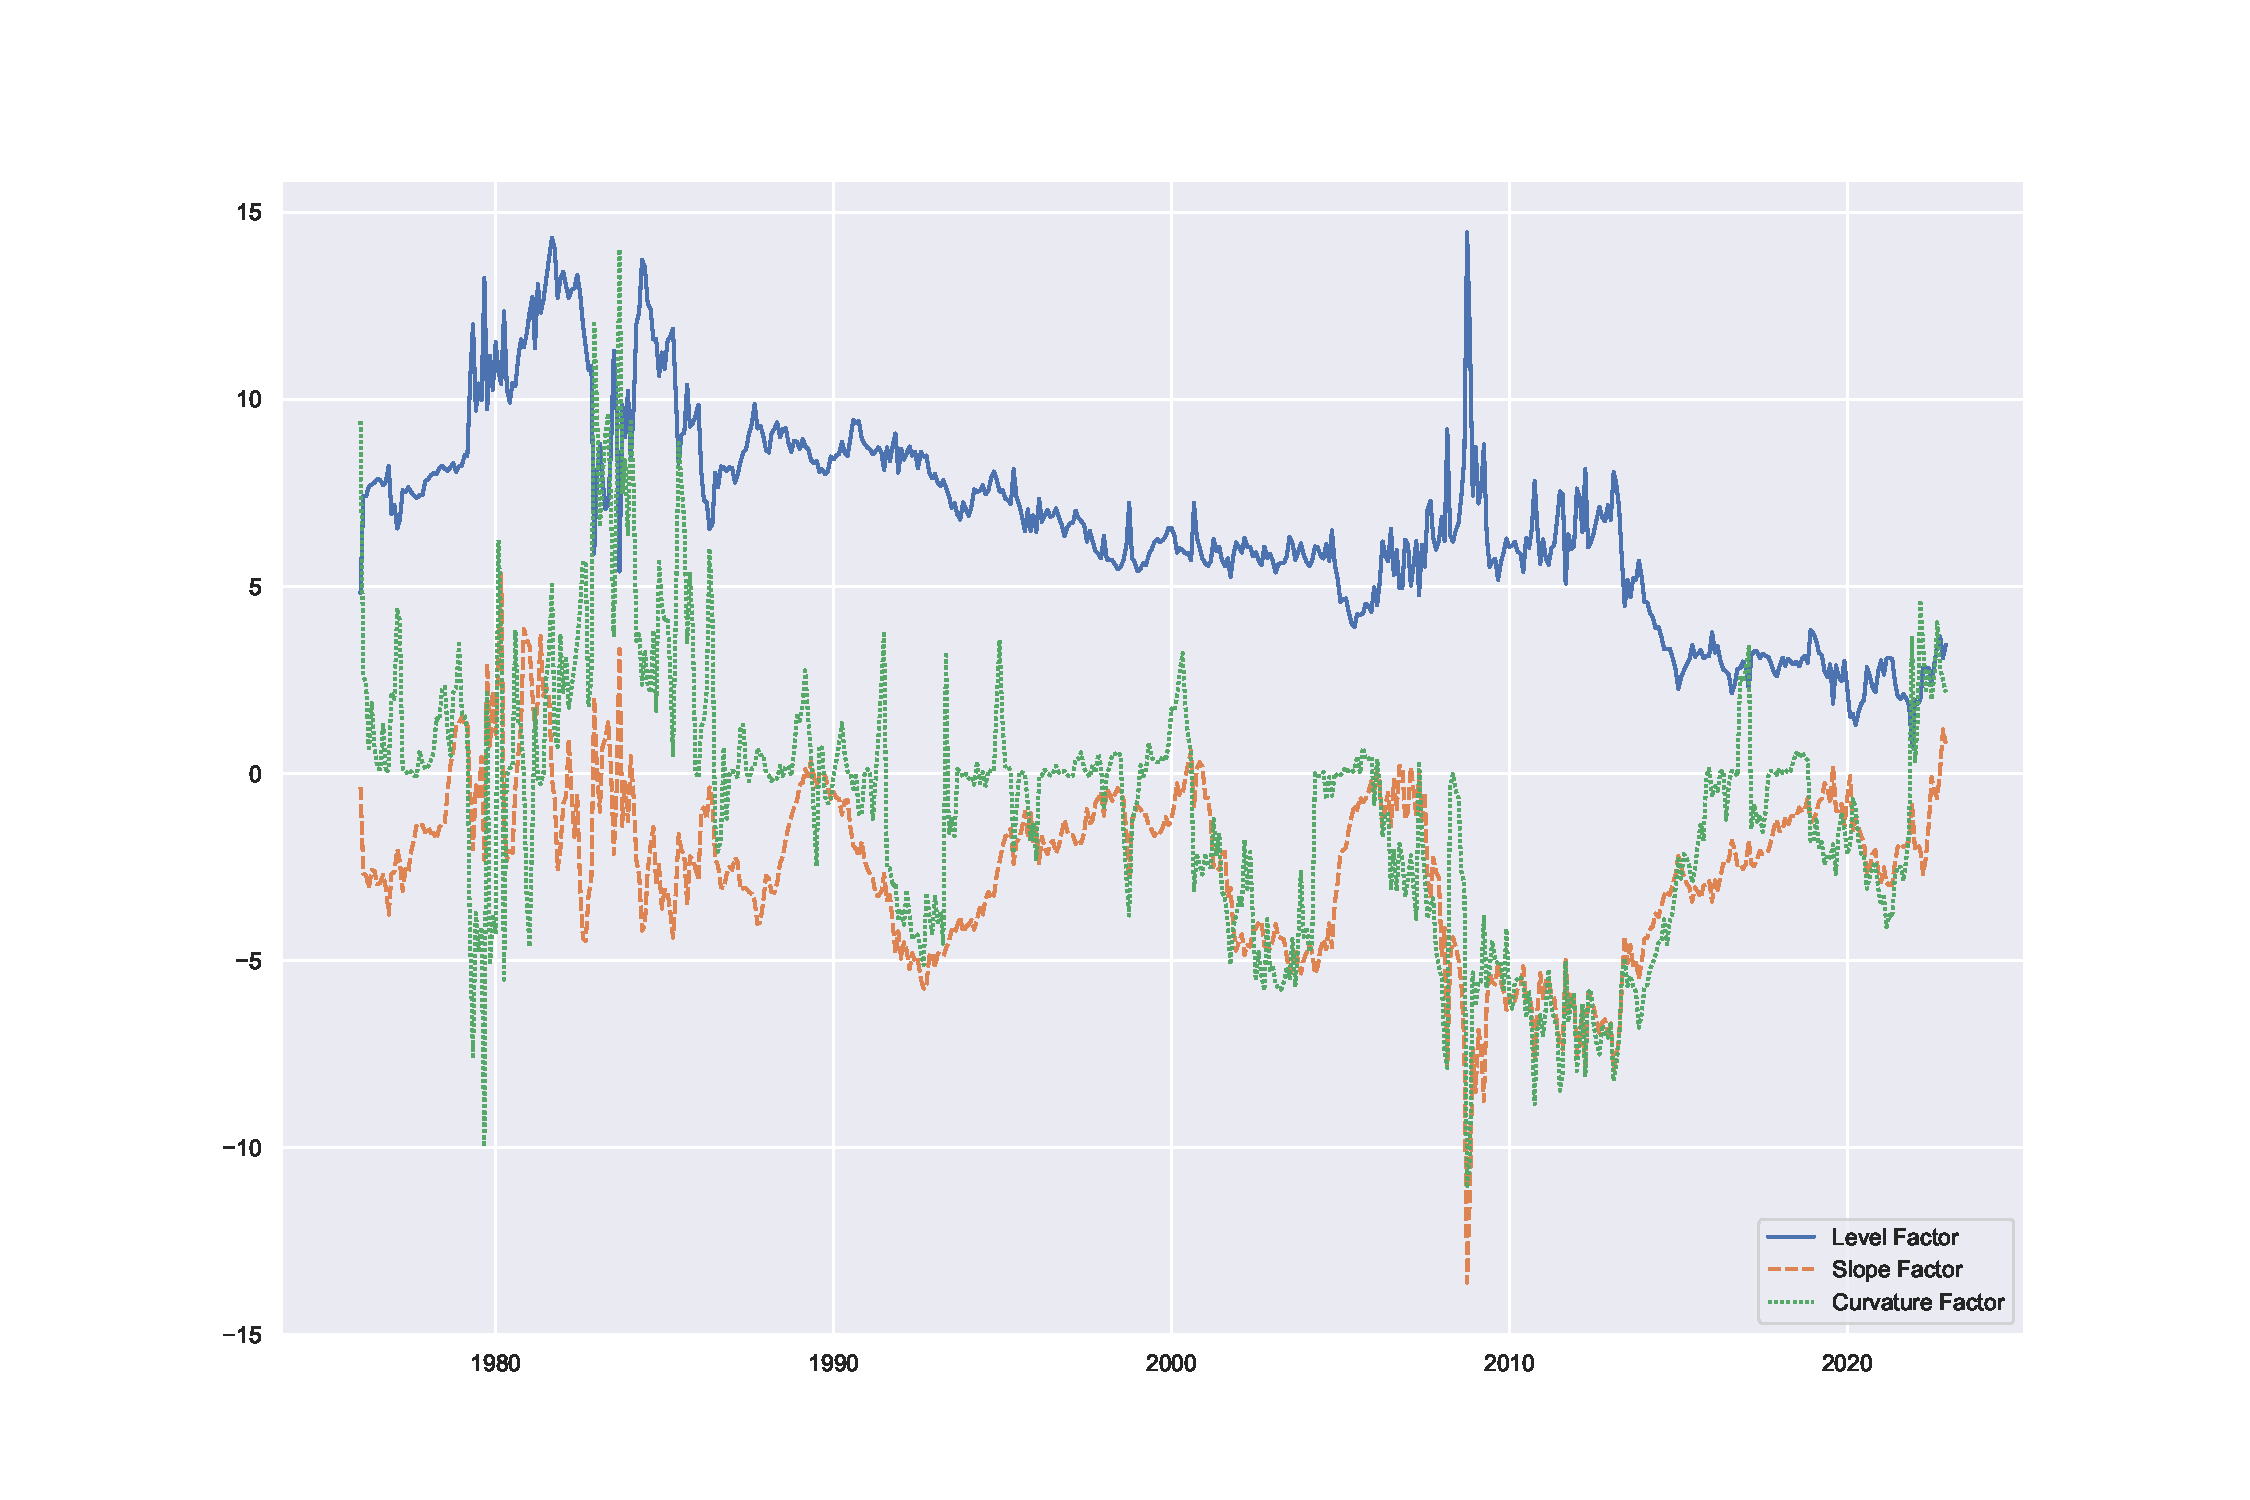
\includegraphics[width=15cm]{Figures/Factor_Figure.pdf}
    \caption{Estimated level, slope and curvature factor, USA (in \%)}
    \label{fig:factors_us}
\end{figure}

In order to get an initial sense of comparability, Figure \ref{fig:factors_us} depicts all three estimated yield curve factors obtained via the Nelson-Siegel model for the US from January 1973 until December 2022.
Among other things, one can see that the level factor, $\hat{L}^{US}_{t}$, has consistently been positive and well above the level of 5\% for most of the time. 
Being above 10\%, the estimated level factor is fairly high during the second oil price crisis induced by the Iranian Revolution in 1979, which caused world oil prices and thus, also US inflation to spike - an interesting observation that is further discussed when looking at Figure \ref{fig:level_factor_us}. 
The spike in October 2008 could potentially be attributed to the onset of the financial crisis, where the bursting of the real estate bubble in the US led to the biggest financial crisis since the Great Depression - an idiosyncratic shock that might reveal possible shortcomings of the Nelson-Siegel model during times of turmoil. 
Though a decreasing trend in the estimated level can be observed since the 1990s, the pace of the decrease has been the highest with the level being the lowest during the 2010s - a time marked by QE and deflationary risks. 
As for the estimated slope ($\hat{S}^{US}_{t}$) and the curvature ($\hat{C}^{US}_{t}$) factors, both factors assume positive and negative values during the sample period. 
It is apparent that the curvature factor is the most volatile, especially during the 1970s and 1980s, while from the 2000s onwards, the correlation between the slope and the curvature factors is fairly high\footnote{The correlation between estimates of the slope and curvature factor is about 32\% from 01-1973 until 12-1999, while it is around 77\% from 01-2000 until the end of the sample}. 
As a mirror image to the likely erroneous spike of the level factor during the financial crisis of 2008, the (negative) slope factor displays a similar spike, only downwards, which, since one would expect an inverted yield curve and thus, an increase of the negative slope at times of a looming a recession, contradicts economic theory as well as countless empirical analyses outlined in the literature review of section \ref{sec:lit_rev}, again underlining the possible inaptitude of the Nelson-Siegel approach when faced with an idiosyncratic event.  

\begin{figure}[!t]
    \centering
    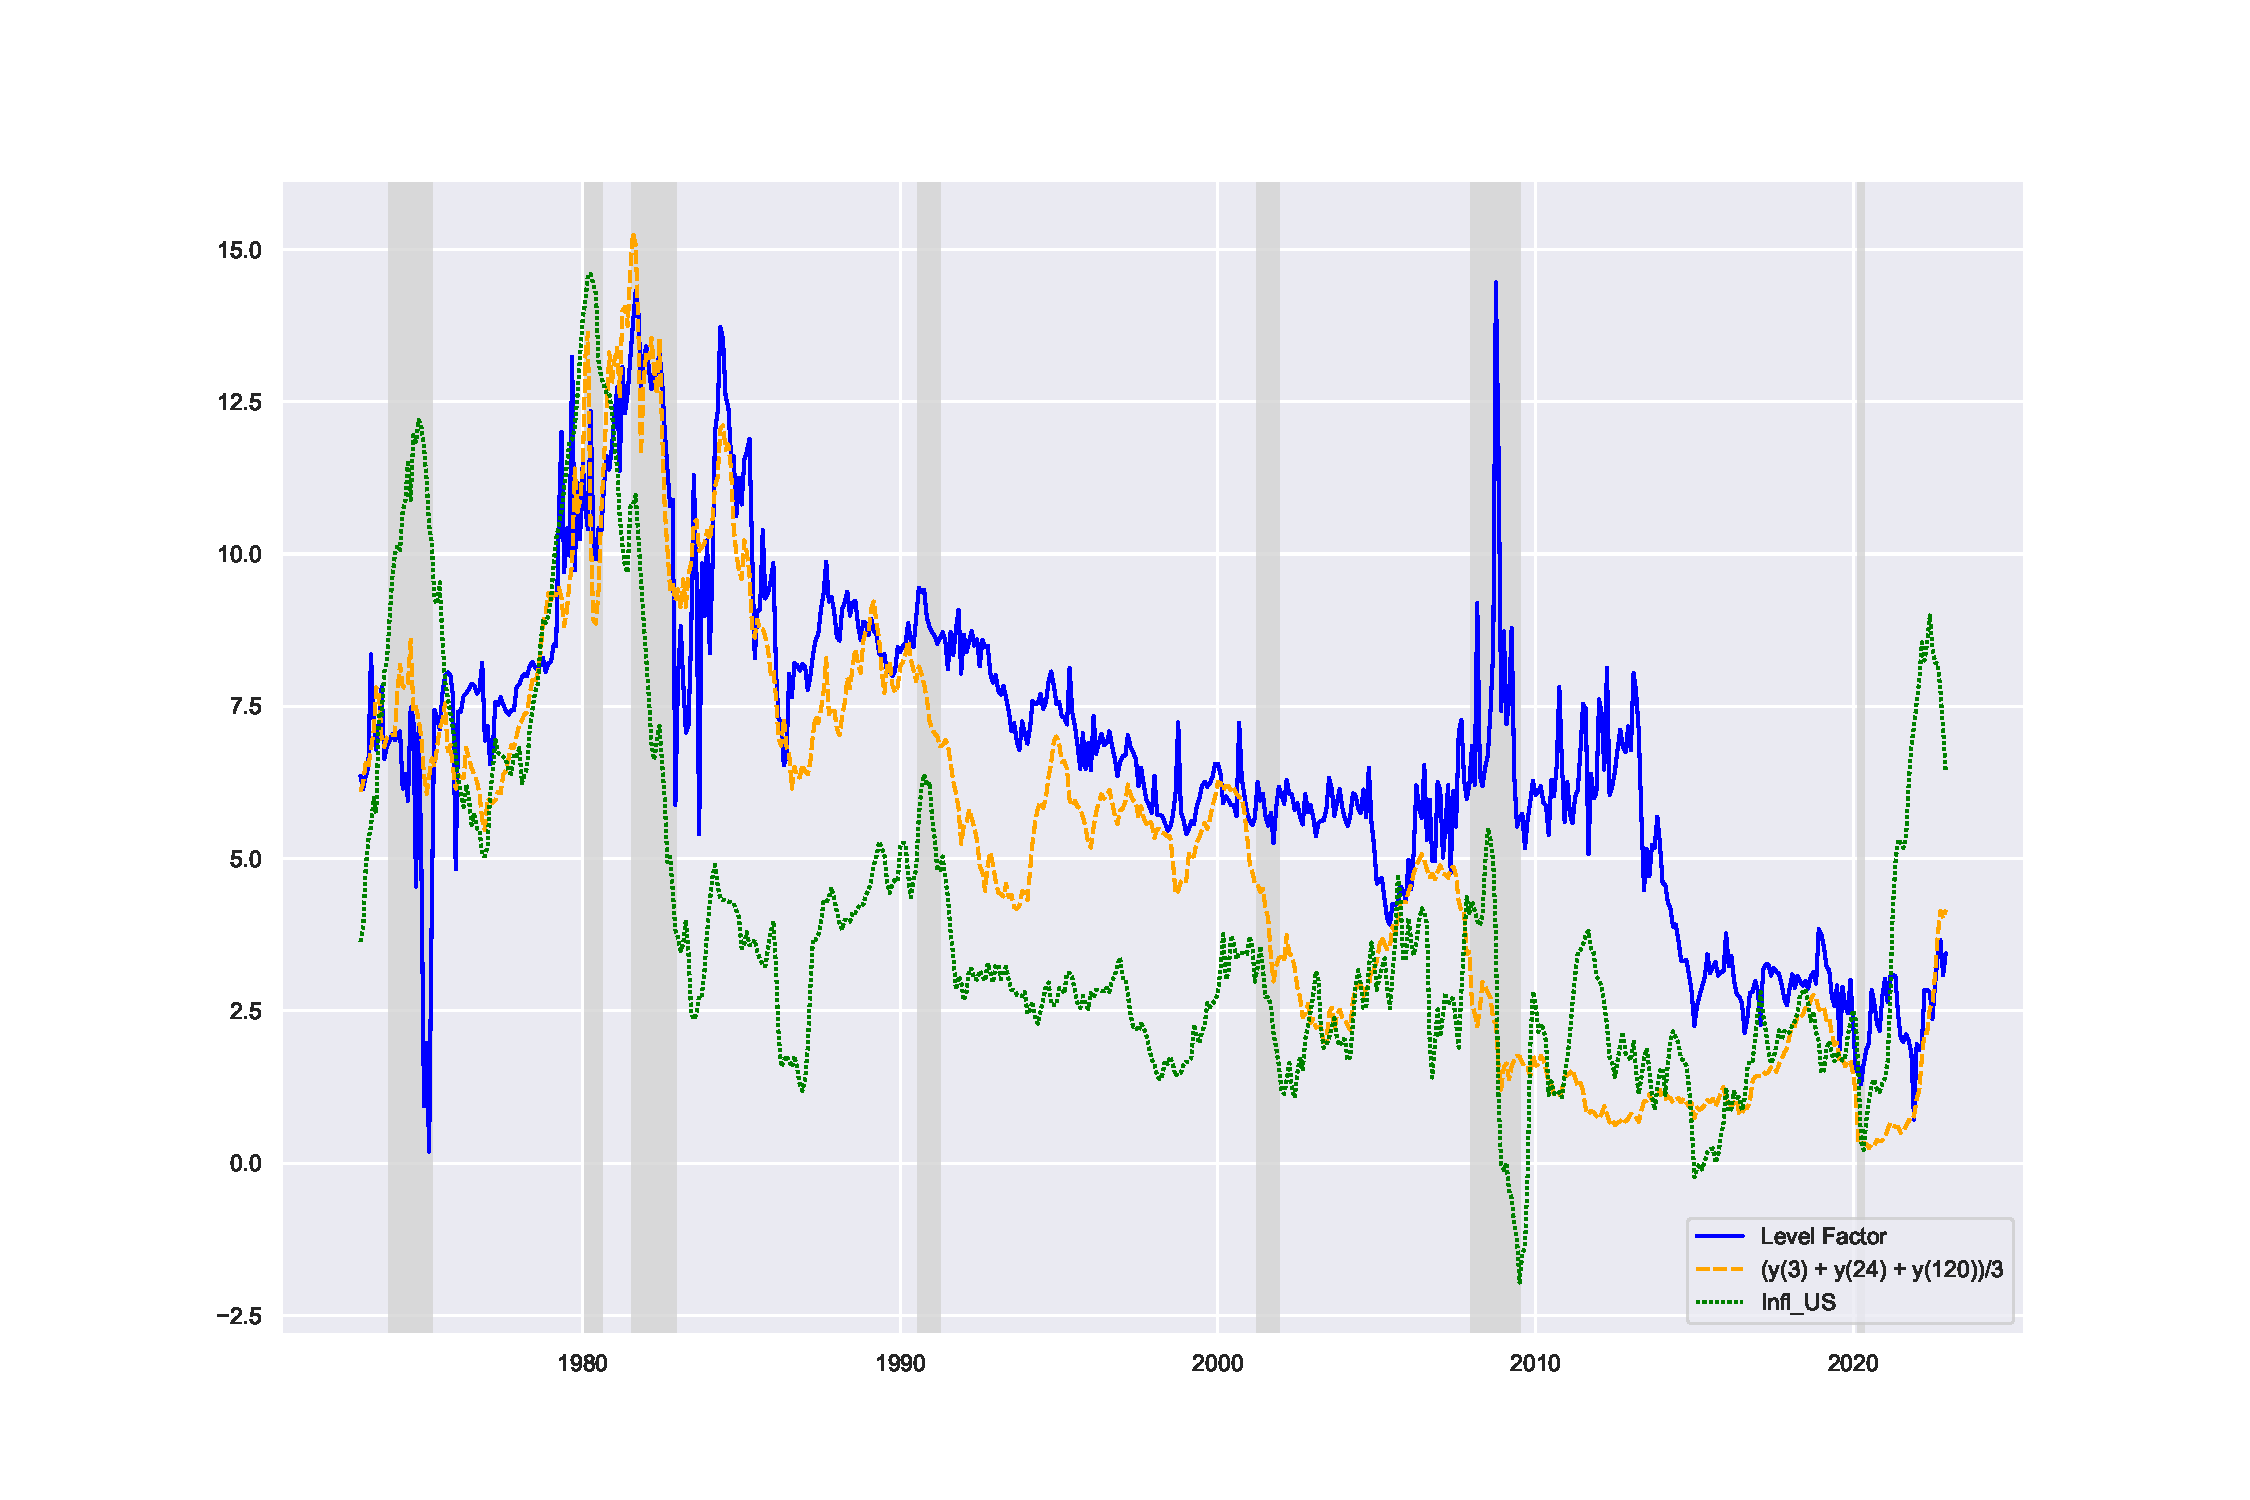
\includegraphics[width=15cm]{Figures/Beta_0_Figure.pdf}
    \caption{Level factor, empirical proxy and inflation, USA (in \%)}
    \label{fig:level_factor_us}
\end{figure}

\begin{figure}[!t]
    \centering
    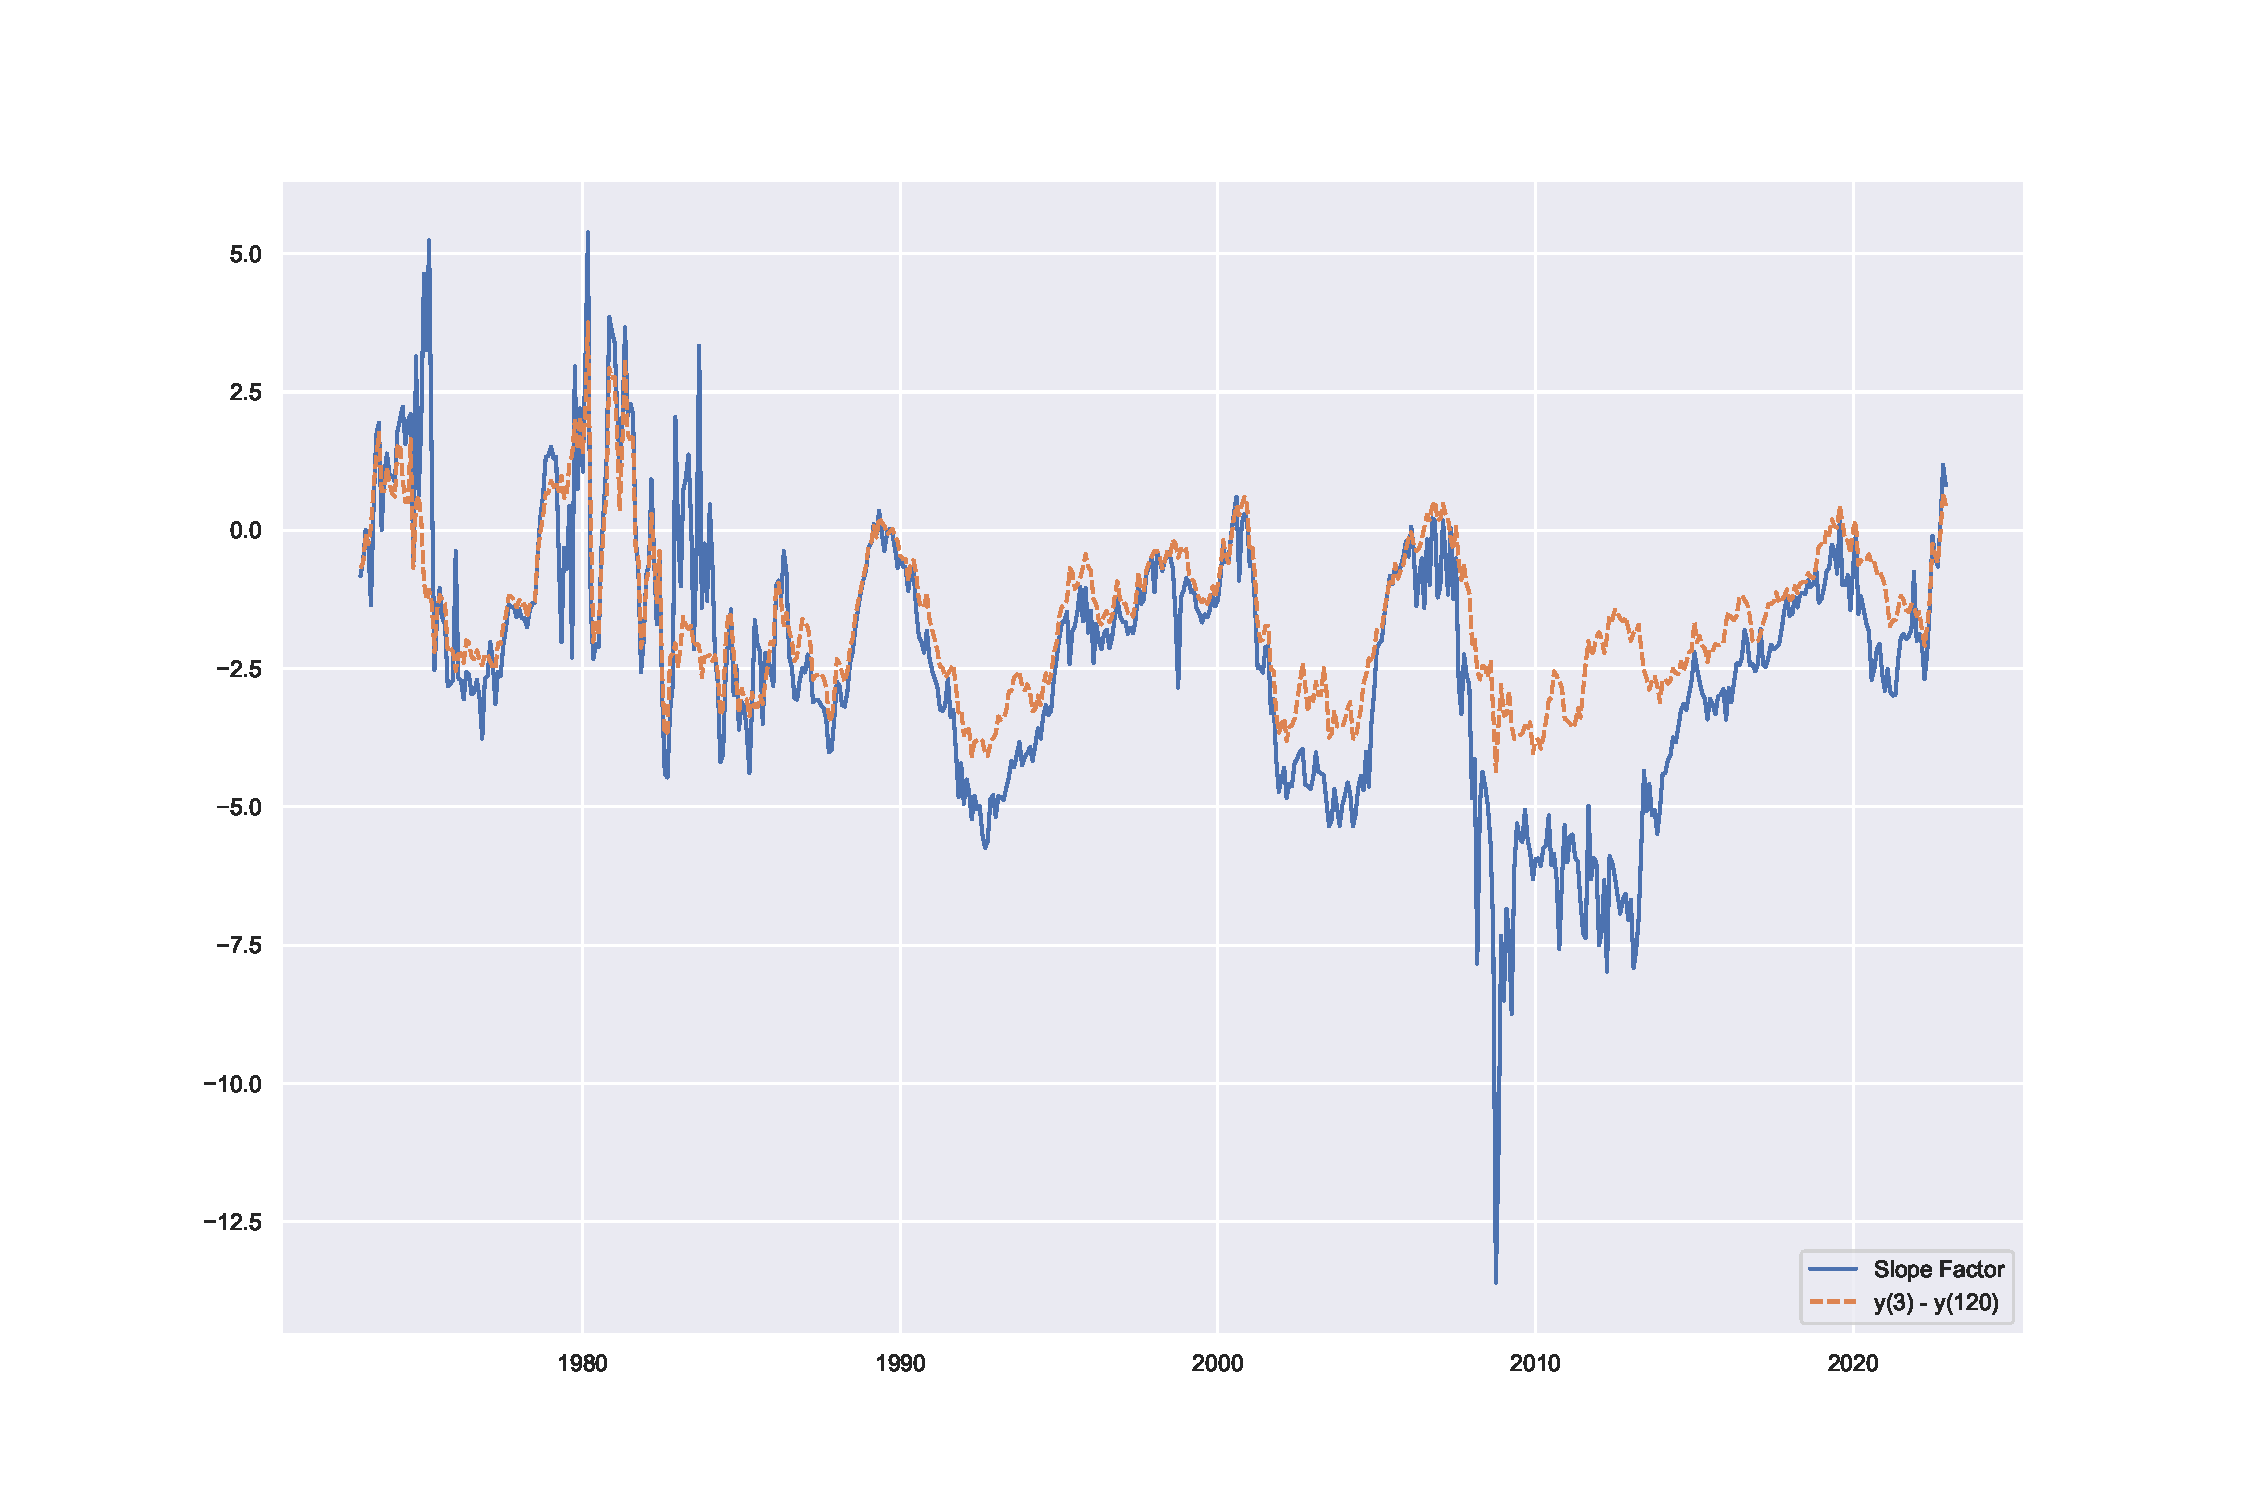
\includegraphics[width=15cm]{Figures/Beta_1_Figure.pdf}
    \caption{Slope factor and empirical proxy, USA (in \%)}
    \label{fig:slope_factor_us}
\end{figure}

% Following \citet{diebold2006macroeconomy}, 
Figures \ref{fig:level_factor_us}-\ref{fig:curvature_factor_us} show the estimated factors together with their empirical proxies. 
These proxies are insofar relevant as they offer a first indication of the gap between the estimated coefficients and the actually realized yields \citep{kanjilal2011macroeconomic}.
Figure \ref{fig:level_factor_us} depicts the estimated level factor, $\hat{L}^{US}_{t}$ and the proxy variable proposed in the literature being the arithmetic average of the 10-year, 2-year and 3-month yield. 
It is apparent that the empirical proxy is fairly close to the estimated level factor, especially in the beginning of the sample, while a stronger divergence can be observed from the financial crisis onwards, though the level proxy has been close to the estimate in recent years. 
Over the whole sample period, the correlation between the estimated level factor and the respective proxy is 82\%, being in line with the findings of \citet{rudebusch2008macro}, and validating the estimate as being a good representation for level factor, i.e. the long-run component of the yield curve. 
Since it is the first indication of a link between the macroeconomy and the yield curve, a highly interesting observation for the task at hand can also be drawn when comparing the level factor with the inflation rate over time. 
From the Fisher equation one can derive how nominal interest rates and inflation expectations could be linked. 
Based on \citet{fisher1930theory}, one would expect that nominal interest rates move one-to-one with a change in expected inflation, with the real interest rate being unaffected. 
In order to study this proposition Figure \ref{fig:level_factor_us} also includes the year-on-year change in the CPI via the dotted green line.
Though this inflation measure is concerned with actual and not expected inflation, one can see the spikes in the inflation rate during the second oil crisis beginning in 1979, where both inflation and the level factor have increased tremendously - a first indication that the inflation rate is indeed linked with the long-run factor of the yield curve. In a similar fashion, $\hat{L}^{US}_{t}$ first spikes in October 2008 and then decreases strongly, a pattern that is almost perfectly coinciding with the inflation rate during that time. 
% Interestingly, this is not observed during the first oil crisis of the 1970s.
When looking at the recent period of inflationary pressures induced by supply bottlenecks during the COVID-19 pandemic in 2021 as well as the Russian aggression in Ukraine in 2022, one can see that again the level factor, which has of course been flanked by increasing interest rates through monetary tightening by the FED beginning in 2022, has moved in accordance with actual inflation, though not rising as sharply as the inflation rate. 
Overall, the estimated level factor and inflation exhibit a rather strong co-movement in the US.
In fact, the correlation between $\hat{L}^{US}_{t}$ and inflation over the sample period is 44\% and significant\footnote{From hereon, a significance level of 5\% is postulated with regards to statistical hypothesis testing}, a finding that is consistent with the interpretation of the level factor as being related to inflation expectations, as described in, among others, \citet{dewachter2006macro}, \citet{rudebusch2008macro}, and \citet{diebold2006macroeconomy}.
% - a first indication that there indeed is a relationship between macro variables and the yield curve.   


% \textbf{Describe why Inflation and Level Factor correlate with each other (see \citet{diebold2006macroeconomy, dewachter2006macro, rudebusch2008macro})}

\begin{figure}[!t]
    \centering
    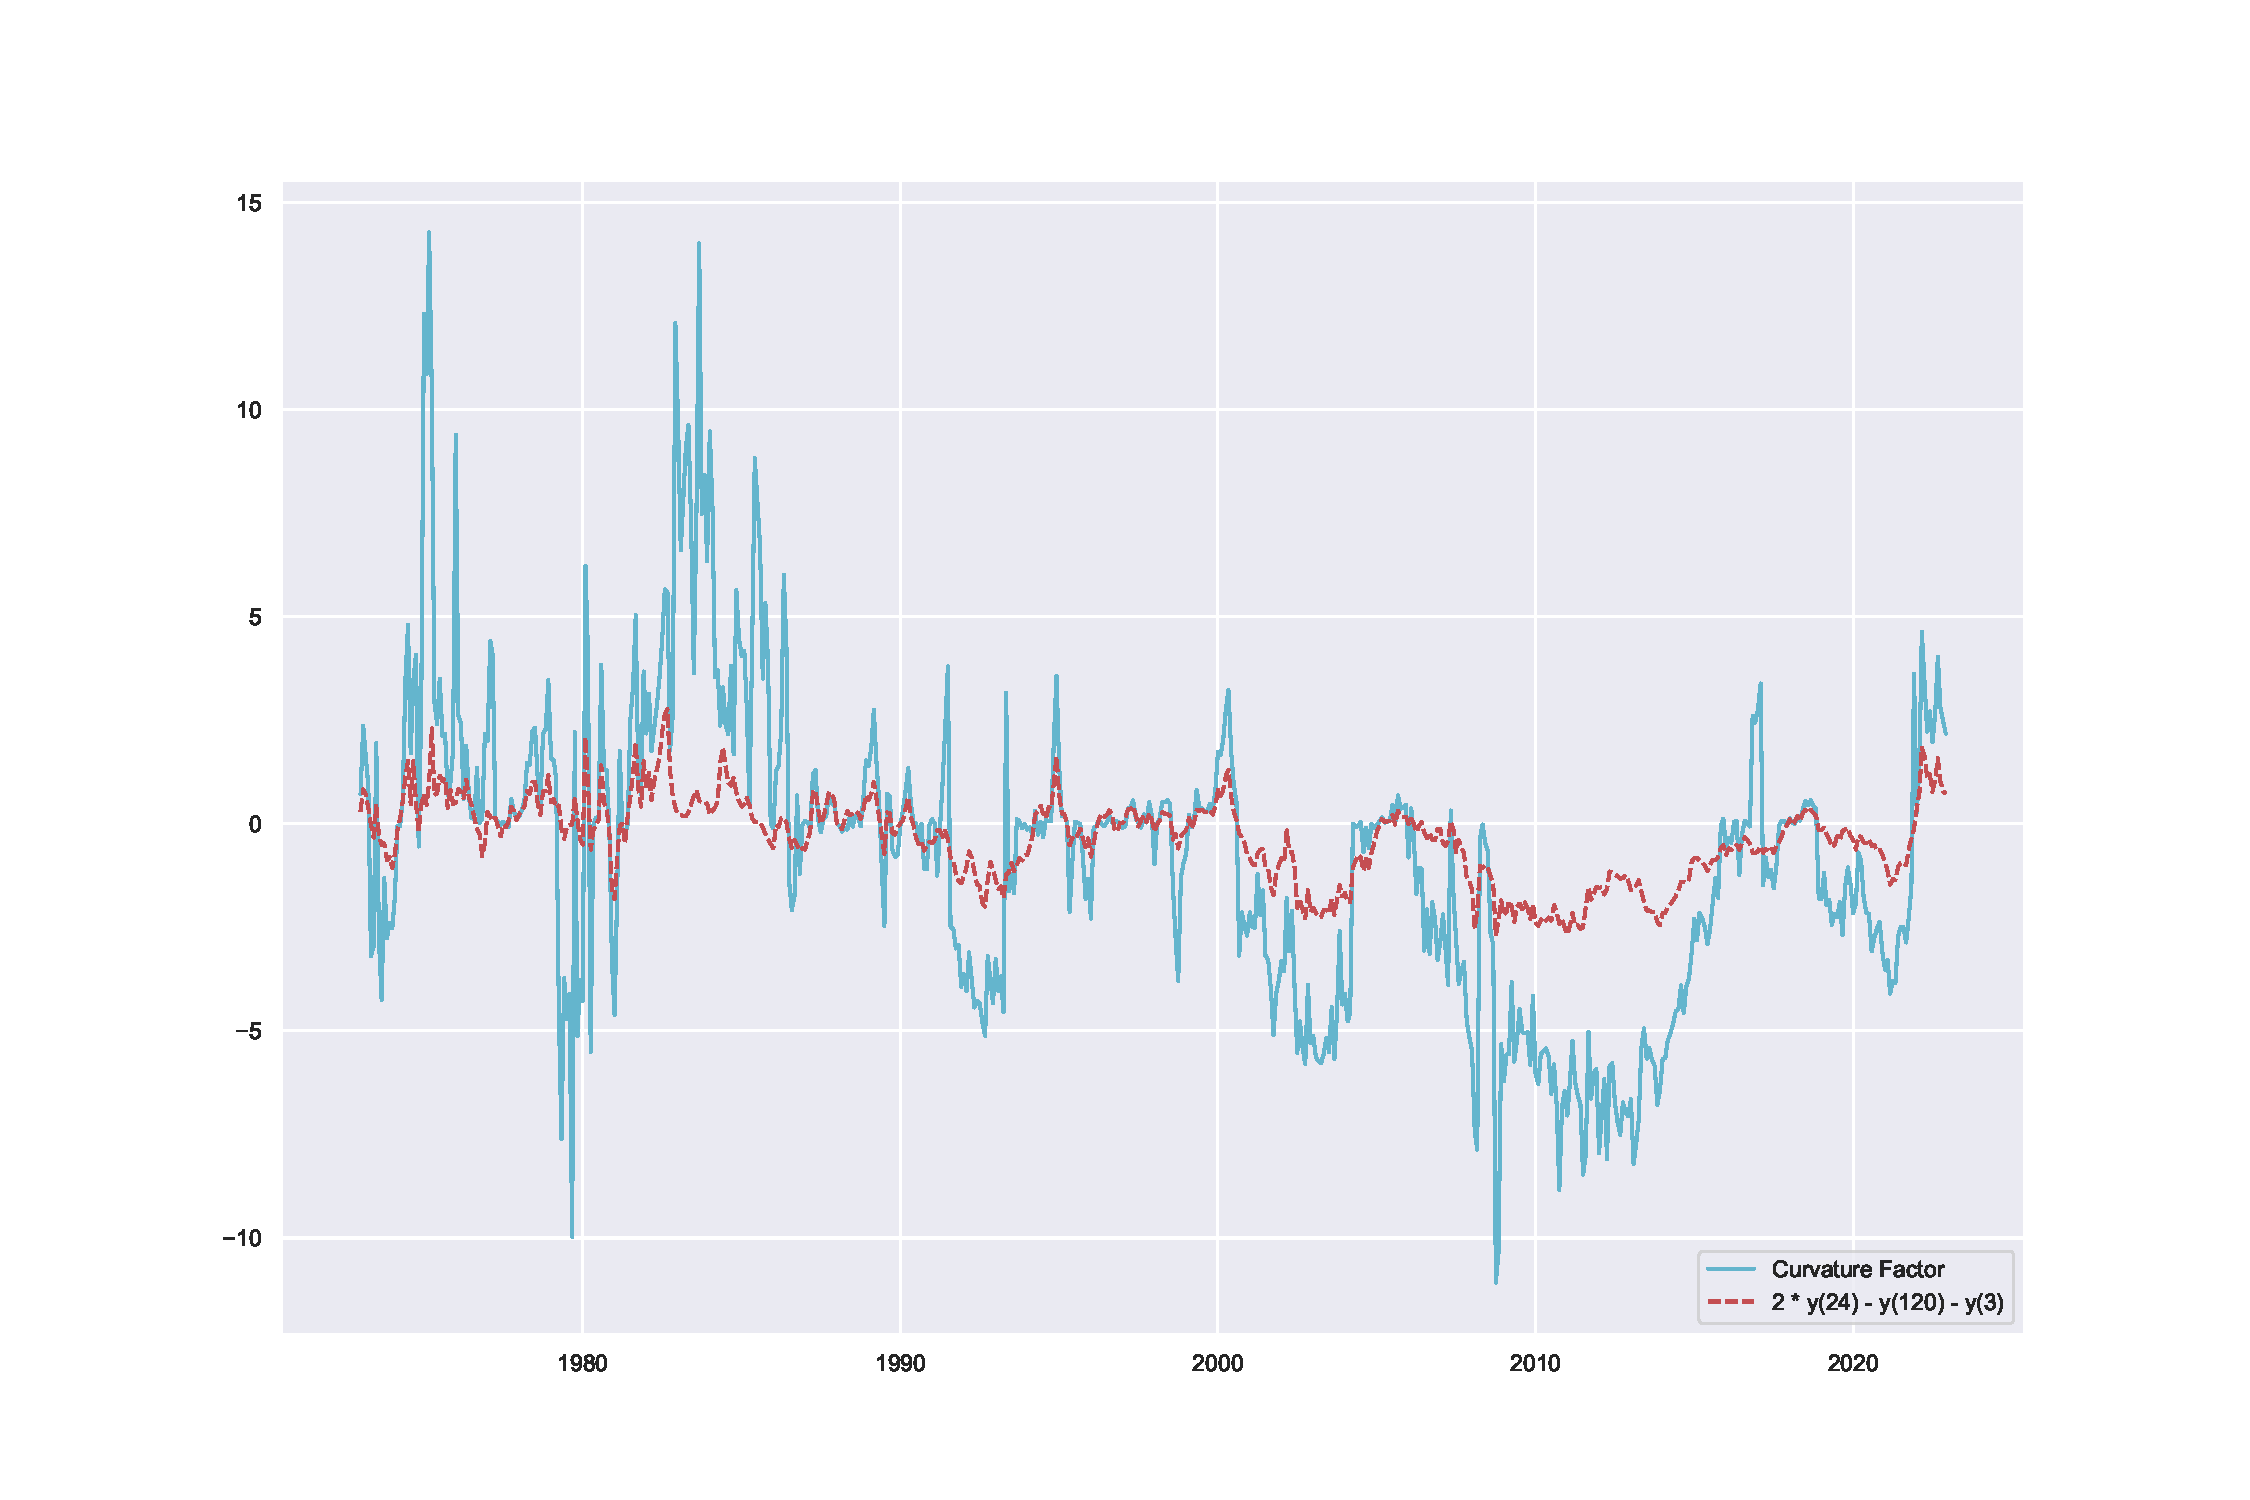
\includegraphics[width=15cm]{Figures/Beta_2_Figure.pdf}
    \caption{Curvature factor and empirical proxy, USA (in \%)}
    \label{fig:curvature_factor_us}
\end{figure}

% \textbf{Correlation between factors, and approximations}

Looking at Figure \ref{fig:slope_factor_us}, one can see that the estimated slope factor, $\hat{S}^{US}_{t}$ is extremely close to its empirical proxy being the (negative) slope of the yield curve, i.e. the difference between the 3-month and 10-year yield. 
In fact, the correlation is strikingly high and significant with 81\%.  
As often done in the literature, the slope factor is said to be correlated, in fact, even able to predict economic activity. 
Thus, to again get a glimpse of a possible link between the macroeconomy and the yield curve represented by the slope factor, Figure \ref{fig:slope_factor_us} also depicts economic activity in the form of the year-on-year growth rate industrial of production over time. 
Evidently, there is some co-movement between the slope and industrial production, where most economic downturns are preceded by an upward spike in the term spread, corroborating the findings related to the yields-to macro literature outlined in section \ref{sec:lit_rev} and again strengthening the case of a link between the yield curve and the macroeconomy. 
% though this pattern is by no means very strong.
% \footnote{Note that the choice of the variable for economic activity matter tremendously. When correlating the estimated slope factor with capacity utilization}.
Similarly in Figure \ref{fig:curvature_factor_us}, with a correlation of 79\%, the curvature factor tends to be somewhat close to its proxy, where they generally have similar trends over time, though it unambiguously has a very high volatility relative to it's proxy variable. 

In summary, on the one hand the observations described above tend to validate the indication that the estimated Nelson-Siegel factors accurately represent the yield curve and are thus, fitted for studying the relationship between the macroeconomy and the term structure. On the other hand, Figures \ref{fig:level_factor_us} and \ref{fig:slope_factor_us} have also offered preemptive evidence confirming that there indeed seems to be a relationship consistent with economic theory as well as the literature, namely that the level factor seems to indeed be an accurate representation of the bonds market long-run inflation gauge, as well as an increasing slope factor potentially indicating an upcoming recession.
% , where evidence for the latter seems to be .  

\begin{table}[t]
    \centering
    \begin{tabular}{lrrr}
        \toprule
        {} &  t-Statistic &  Critical value &  p-value \\
        \midrule
        $IP^{US}_{t}$  &      -5.6906 &         -2.8665 &   0.0000 \\
        $\pi^{US}_{t}$ &      -3.0096 &         -2.8665 &   0.0340 \\
        $i^{US}_{t}$   &      -2.7681 &         -2.8665 &   0.0630 \\
        $FS^{US}_{t}$  &      -5.4727 &         -2.8664 &   0.0000 \\
        $\hat{L}^{US}_{t}$   &      -1.7930 &         -2.8665 &   0.3839 \\
        $\hat{S}^{US}_{t}$   &      -3.0791 &         -2.8665 &   0.0281 \\
        $\hat{C}^{US}_{t}$   &      -2.9236 &         -2.8665 &   0.0427 \\
        $M^{US}_{t}$   &      -4.8305 &         -2.8665 &   0.0000 \\
        \bottomrule
    \end{tabular}
    \caption{Augmented Dickey-Fuller (ADF) unit root test, US}
    \label{tab:adf_us}
\end{table}

% In order to further understand the interactions between the yield curve and the macroeconomy on an econometric basis,

Consequently, the next step involves analysing macroeconomic and yield curve variables together in a comprehensive structural VAR framework\footnote{Note that the VAR models in this thesis are estimated via Ordinary Least Squares (OLS)} outlined in section \ref{sec:method}. 
However, before fitting a VAR model, it is first important to understand the nature of the variables involved. Thus, Table \ref{tab:adf_us} shows the results of an Augmented Dickey-Fuller test of each variable included in the model, testing whether it is stationary, i.e. it possesses a unit root at the 5\% significance level. 
Apart from the Federal Funds rate ($i^{US}_{t}$) and the level factor ($\hat{L}^{US}_{t}$), one can reject the null hypothesis of the existence of a unit root at the 5\% level for all remaining model variables. 
This is insofar not surprising given the fact that the year-on-year growth rates for industrial production, the price level and stock prices are used, which results in detrended time-series. 
Taking the first differences of both the Federal Funds rate as well as the level factor would result in stationary time series, though due to consistency considerations as well as previous methodologies used in the literature, both time series are included in levels. 
As noted by \citet{morales2010real}, due to parsimony reasons, the order of the vector autoregression process is selected based on both the Bayesian (BIC) and Hannan-Quinn (HQIC) information criteria selecting a lag length of 1. 
Table \ref{tab:VAR_output_US_v2} presents the estimated VAR(1) coefficients of the comprehensive yields-macro model along with the log-likelihood and various information criteria. 
Looking at the individual time series on the main diagonal, one can immediately infer that the three yield curve factors are highly persistent, especially the level and slope factor, while in the macroeconomic realm industrial production and inflation display a high persistence. 
Additionally, the financial market variables stock prices as well as financial stress exhibit a high persistence.  
Only the short-term interest rate has a strikingly low persistence, which can be seen as confirming the finding by \citet{rudebusch2005monetary} that incorporating the term structure when modelling the monetary policy reaction function results in refuting the notion of monetary policy inertia. 
% When examining the off-diagonal estimated coefficients
% In spite of these findings, the off-diagonal interactions are better suited for impulse response analysis

% \textbf{Describe significance of estimates}

% \textbf{FFR monetary policy instrument?}

% \textbf{Monetary Policy intertia reason for low persistence?}

% \textbf{passt ordering? Ev Financial stress weiter nach unten (so wie stock market)}

Since the aim of this thesis is to understand the dynamic interactions
% , i.e. the off-diagonal elements of interest,
between the yield curve and the macroeconomy in the United States, Figure \ref{fig:IRF_US} depicts the orthogonal impulse responses over a period of three years (36 months) with 90\% confidence intervals. 
Each row shows the response of a certain variable $i$ to a specific structural shock of variable $j$, where each column displays to which variable $j$ the respective shock occurred. 
For example, the second row shows the responses of inflation ($\pi^{US}_{t}$) to various structural shocks to the model variables, while the third column illustrates the responses of each variable to a structural monetary policy shock in the form of the short-term interest rate ($i^{US}_{t}$). 
With this in mind, there are four types of impulse responses to consider: macro-to-macro, macro-to-yields, yields-to-macro and yields-to-yields.  


% \textbf{cite papers that depict the price puzzle}

\begin{sidewaystable}
    \centering
\begin{tabular}{lrrrrrrrr}
        \toprule
        {} &        $IP^{US}_{t}$ &   $\pi^{US}_{t}$ &       $i^{US}_{t}$ &       $FS^{US}_{t}$ &         $\hat{L}^{US}_{t}$ &         $\hat{S}^{US}_{t}$ &         $\hat{C}^{US}_{t}$ &   $M^{US}_{t}$ \\
        \midrule
    const & -0.1651 & 0.2026 & -0.0501 & -0.0345 & 0.5002 & -0.5581 & -0.7174 & 1.5318 \\
     & (0.1744) & (0.0529) & (0.0471) & (0.0318) & (0.1138) & (0.1314) & (0.2473) & (0.6817) \\
    $IP^{US}_{t-1}$ & 0.8816 & 0.0132 & 0.0086 & 0.0005 & 0.0046 & 0.0025 & -0.0134 & -0.4305 \\
     & (0.0137) & (0.0042) & (0.0037) & (0.0025) & (0.0089) & (0.0103) & (0.0194) & (0.0535) \\
    $\pi^{US}_{t-1}$ & -0.0477 & 0.9795 & 0.0126 & 0.0058 & 0.0102 & 0.0223 & 0.0039 & -0.4072 \\
     & (0.0260) & (0.0079) & (0.0070) & (0.0047) & (0.0169) & (0.0196) & (0.0368) & (0.1014) \\
    $i^{US}_{t-1}$ & -0.2730 & -0.0024 & 0.5393 & 0.0220 & -0.0801 & -0.0106 & 0.3227 & -0.1502 \\
     & (0.0632) & (0.0192) & (0.0171) & (0.0115) & (0.0413) & (0.0476) & (0.0897) & (0.2471) \\
    $FS^{US}_{t-1}$ & -0.6609 & -0.1468 & 0.0521 & 0.8966 & 0.0685 & -0.1480 & -0.2175 & -4.4019 \\
     & (0.1260) & (0.0382) & (0.0340) & (0.0230) & (0.0822) & (0.0949) & (0.1787) & (0.4925) \\
    $\hat{L}^{US}_{t-1}$ & 0.3604 & -0.0011 & 0.5155 & -0.0237 & 1.0214 & 0.0493 & -0.2522 & 0.5345 \\
     & (0.0739) & (0.0224) & (0.0199) & (0.0135) & (0.0482) & (0.0557) & (0.1048) & (0.2888) \\
    $\hat{S}^{US}_{t-1}$ & 0.2571 & 0.0431 & 0.5407 & -0.0305 & 0.1206 & 0.9161 & -0.2928 & 0.4040 \\
     & (0.0734) & (0.0223) & (0.0198) & (0.0134) & (0.0479) & (0.0553) & (0.1041) & (0.2869) \\
    $\hat{C}^{US}_{t-1}$ & 0.0303 & -0.0163 & -0.0158 & 0.0035 & 0.0426 & -0.0156 & 0.8149 & -0.0219 \\
     & (0.0191) & (0.0058) & (0.0052) & (0.0035) & (0.0125) & (0.0144) & (0.0271) & (0.0747) \\
    $M^{US}_{t}$ & 0.0148 & -0.0030 & -0.0009 & 0.0001 & 0.0001 & -0.0013 & 0.0049 & 0.9086 \\
     & (0.0040) & (0.0012) & (0.0011) & (0.0007) & (0.0026) & (0.0030) & (0.0057) & (0.0157) \\
    \midrule
    Log-Likelihood & -5443.2304 \\
    AIC & -4.2882 \\
    BIC & -3.7599 \\
    HQIC & -4.0825 \\
    \bottomrule
    \end{tabular}
    \caption{Vector Autoregression estimation results, US}
    \label{tab:VAR_output_US_v2}
\end{sidewaystable}

\begin{sidewaysfigure}
    \centering
    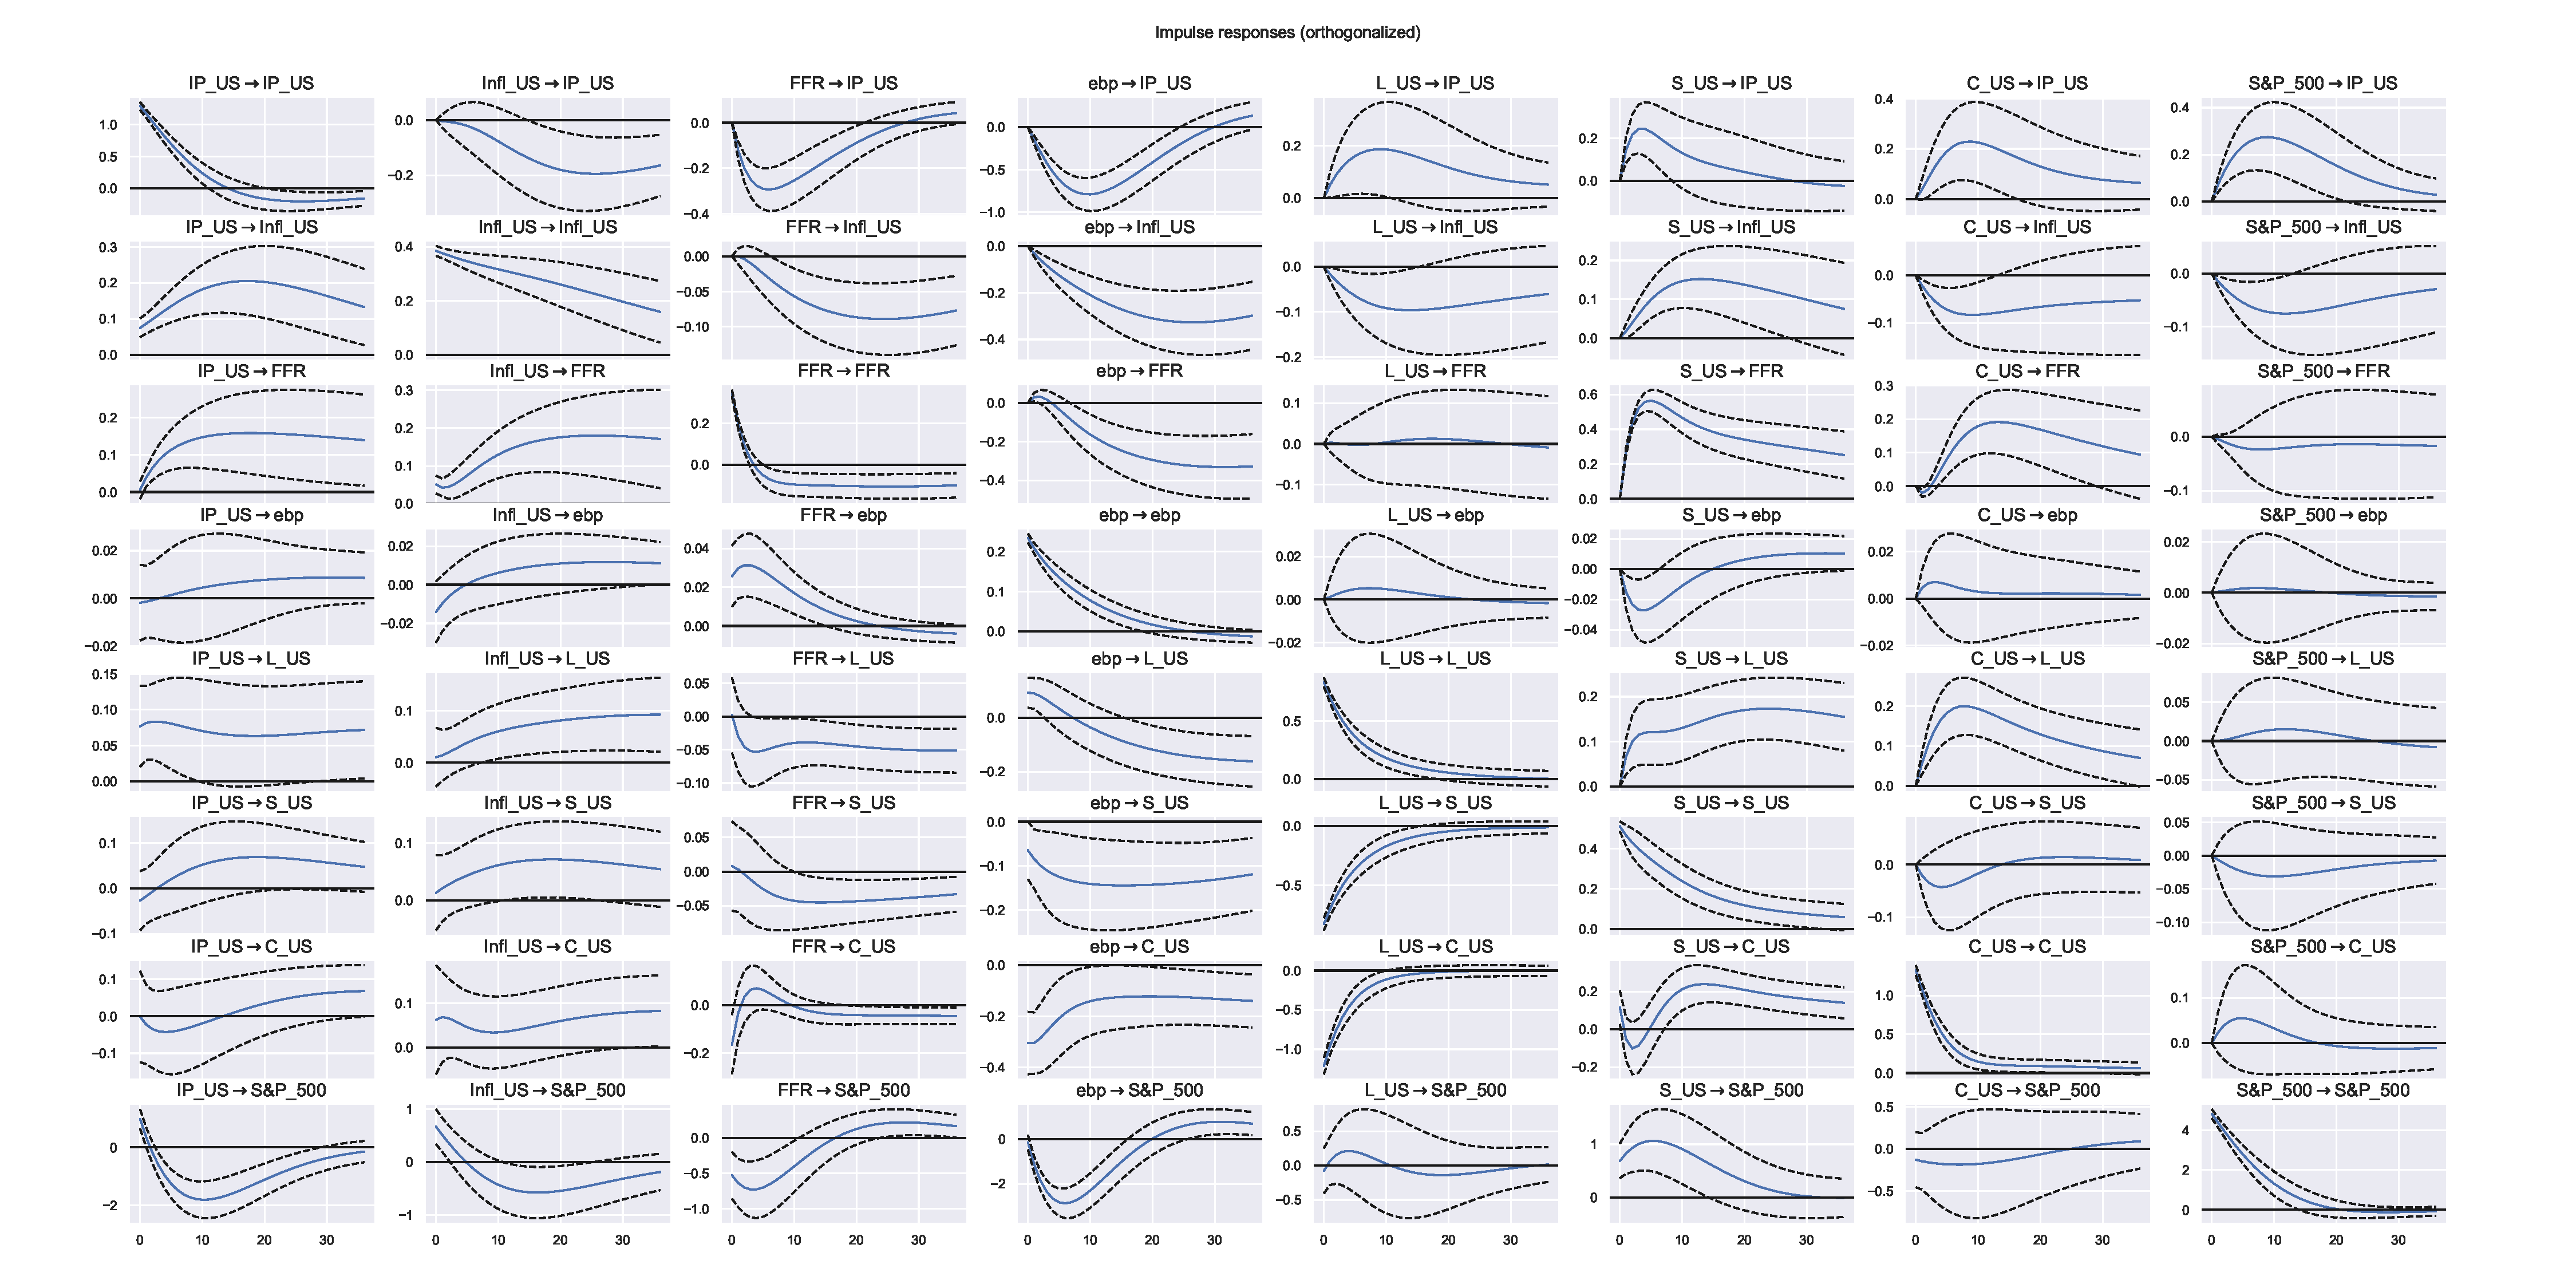
\includegraphics[scale=0.29]{Figures/IRF_US_30_15_v2.pdf}
    \caption{Impulse Responses, US}
    \label{fig:IRF_US}
\end{sidewaysfigure}


As a first assessment of validity, the macro-to-macro impulse responses are considered. 
It is reassuring that the results seem to broadly match those of similar small scale macro models oftentimes used in the literature (e.g. \citet{gali_1992}, \citet{stock2001vector}). 
Specifically, a shock to industrial production, i.e. an aggregate demand shock, increases both inflation (second row, first column) and the short-term interest rate (third row, first column), while an inflation shock decreases aggregate demand over time. 
The Federal Funds rate increases on impact as well as over time to a positive inflation shock, which is not only consistent with economic theory, but, given the dual mandate of the FED, also with real-world central bank behavior.
% , e.g. modelled by central bank reaction functions. 
The last macro-to-macro shock to consider is a monetary policy shock (third column). 
Since the short-term restrictions described in chapter \ref{sec:method} are based on the assumption that both industrial production and inflation react with a certain time lag, both variables do not react on impact, but over time - as one would expect based on economic reasoning - industrial production as well as inflation decrease as a response to a surprise increase in the short-term rate, where the decrease of inflation is more persistent, while industrial production decreases more strongly during the first year. 

Examining the first direction of the link between the macroeconomy and the yield curve, i.e. yield curve responses to macro shocks, offers some interesting insights. 
For example, an aggregate demand shock increases the level factor, which, when keeping in mind the interpretation 
% offered by \citet{diebold2006macroeconomy} 
of the level factor as the bond's market long-run inflation expectation - via the Fisher effect - seems reasonable as higher aggregate demand should generally lead agents to expect a higher future price level according to standard economic theory.  
Similarly, the slope factor increases after an aggregate demand shock over time, meaning that the short-end of the yield curve rises relative to the long-end. 
Again, this is in line with standard monetary policy responses to surprises in aggregate demand since bond investors would expect central banks to increase interest rates in the near term as they anticipate higher inflation due to the aggregate demand shock, likely pushing up short-run yields relative to the long-end of the term structure \citep{diebold2006macroeconomy}.
A similar response can be observed when looking at aggregate supply shocks (inflation shocks).
Specifically, the level as well as the slope factor increase to US inflation shocks.
The former result can be explained via the aforementioned Fisher effect, where the bond market likely expects higher future inflation when facing a surprise upward tilt in the current inflation rate leading to an increase in yields. 
The latter effect is again linked to monetary policy, where higher short-term rates are priced in by investors due to present and future expected price level increases, leading to a more negatively sloped yield curve. 
Interestingly, both phenomena have occurred only recently during the last two years where inflationary pressures induced by the war in Ukraine led to significant increases in US yields due to the markets expectation of an imminent monetary tightening by the FED, while the yield curve inverted as short-end yields exceeded long-end yields in anticipation of an upcoming recession. 
The last macro-to-yields shock to consider is a monetary policy shock. 
The level factor decreases as a response to a surprise increase in the Federal Funds rate (third column). 
In this context, contrasting explanations regarding the level factors response to a monetary policy shock are offered. 
Given a central bank has a high degree of credibility and transparency, a surprise monetary tightening could indicate a lower inflation target and thus, induce bond investors to revise their inflation expectations downwards, potentially lowering the level factor, while a surprise tightening could also signal that a central bank is concerned about an overheating economy and an overshooting inflation rate, which would likely result in higher expected inflation and thus, an increasing level factor \citep{diebold2006macroeconomy}. 
Apparently, the former effect has dominated the latter over the sample period, which does not seem implausible given the high credibility of the FED. 

The other direction of causality to consider is the yields-to-macro channel. 
Whereas the short-term interest rate does not react to the long-run level factor, its reaction to the slope factor is strikingly high, confirming that there is a close connection between the monetary policy instrument and the short-run factor of the yield curve. 
Once more, two distinct explanations are offered by the literature. 
On the one hand, the FED might respond to current yields when setting the short-term rate, whilst on the other hand, market yields very likely respond to new information regarding the macroeconomy in anticipation of monetary policy decisions, hence, shifts in fixed-income markets presumably precede central bank actions \citep{diebold2006macroeconomy, morales2010real}.
This would, for example lead to short-end yields to increase in anticipation of an imminent monetary policy tightening.
Another compelling case to consider is a shock to the level factor, which increases aggregate demand. 
This is insofar relevant from the economists lens when once again keeping in mind the level factors interpretation as a proxy for inflation expectations. 
In this case, an increase in inflation expectations lowers the ex-ante real interest rate, $i^{US}_{t} - \hat{L}^{US}_{t}$, leading to a surge in economic activity - a finding that is consistent with standard DSGE models. 
In contrast, some rather implausible responses raise questions about the validity of the yields-to-macro results. 
For example, the response of industrial production to a surprise increase in the yield curve slope does contradict previous findings in the literature. 
Specifically, an increase in the slope - equivalent to a flattening and potentially inversion of the yield curve - is generally associated with an imminent recession rather than an economic boom. 
Similarly, one would anticipate inflation to decrease in response to a shock to the slope factor, whereas it is expected to increase with an increasing level factor, i.e. due to the decreasing ex-ante real interest rate. 
Based on these dubious results regarding the slope one could argue that these findings confirm the conclusions of \citet{ang2006does}, where the short-term interest rate dominates the slope of the yield curve when predicting economic activity, at least when comparing the plausibility of the results for the short-term interest rate vis-a-vis the slope in Figure \ref{fig:IRF_US}. 
% , where the  economic theory as well as previous findings in the literature. 
Furthermore, it could be argued that the modelling strategy based on OLS estimates applied certainly has some limitations and leads to partly improbable results. 

% \textbf{\citet{ang2006does} results regarding slope somewhat confirms their finding that the short rate dominates the slope when predicting economic activity}

Generally, it has to be noted that based on the impulse responses the yields-to macro responses have wider confidence intervals most of the time, hence, it seems that there is more uncertainty involved in the macro responses to yields shocks, whereas there is a stronger evidence for the macro-to-yields channel since those responses are associated with less uncertainty as well as broadly being consistent with economic theory as well as results from the literature. 

The remaining impulse responses to consider are the yields-to-yields shocks. 
Apart from the high persistence in the level and slope factor noted above, some noteworthy observations include the slope factors response to a level factor shock.
Consistent with the findings of \citet{diebold2006macroeconomy}, a surprise increase in the level factor, i.e. long-run inflation expectations, is associated with loose monetary policy conditions represented by a lowering of the short-end of the yield curve relative to the long-end, synonymous with a steepening of the yield curve.
% , i.e. a decrease in the slope factor. 
Similarly, a surprise increase in the slope factor, possibly as anticipation to a monetary tightening, is associated with an increase of the level factor, corresponding to higher future inflation expectations. 



% In order to get an initial quantitative gauge how the yield curve factors and the macro variables are related, Table xxx shows the results of various Granger causality tests conducted for the sample variables. 
% Though Table xxx shows the individual relationships between the model variables, of higher importance for the research question are the 

\begin{table}[!t]
    \centering
    \begin{tabular}{lllll}
    \toprule
    {} &     t-statistic &      Critical value &                 p-value 
    \\
    \midrule
    Macro-to-Yields &  4.3170 &  1.8818 &  0.0000 &  \\
    % \midrule
    Yields-to-Macro &  91.2622 &  1.8818 &  0.0000  \\
\bottomrule
    \end{tabular}
    \caption{Block Granger causality tests, US}
    \label{tab:granger_us}
\end{table}

Finally, the link between the yield curve factors and the macroeconomic variables are assessed using block Granger causality tests, where one can test if a set of variables Granger cause another set of variables in the model. 
Conveniently, this method enables to determine whether there is a one- or bi-directional relationship present, e.g. testing whether solely a set macro variables Granger cause the yield curve factors or if both the macro variables do Granger cause and are Granger caused by the yield curve factors. 
In the present setting, the macro-to-yields test examines whether the set of macro variables in the model ($IP^{US}_{t}$, $\pi^{US}_{t}$, $i^{US}_{t}$) do Granger cause the estimated yield curve factors ($\hat{L}^{US}_{t}$, $\hat{S}^{US}_{t}$, $\hat{C}^{US}_{t}$), whilst the yields-to-macro test evaluates the presence of a Granger causality in reverse order, namely, if the yield curve factors Granger cause the set of macro variables. 
Based on Table \ref{tab:granger_us}, depicting the resulting block Granger causality tests, one can conclude that there seems to be a bi-directional link present in the United States, where both macroeconomic variables seem to contain useful information regarding the behavior of the yield curve and, vice versa, the yield curve seems to affect macroeconomic fluctuations. 

% Thus, the next step involves analysing macroeconomic and yield curve variables together in a comprehensive structural VAR setting outlined in section \ref{sec:method}. Note that the VAR model is estimated via Ordinary Least Squares (OLS).  


\subsection{The Yield Curve and the Macroeconomy in the Euro Area}
\label{sec:analysis_ea}

\begin{figure}[!t]
    \centering
    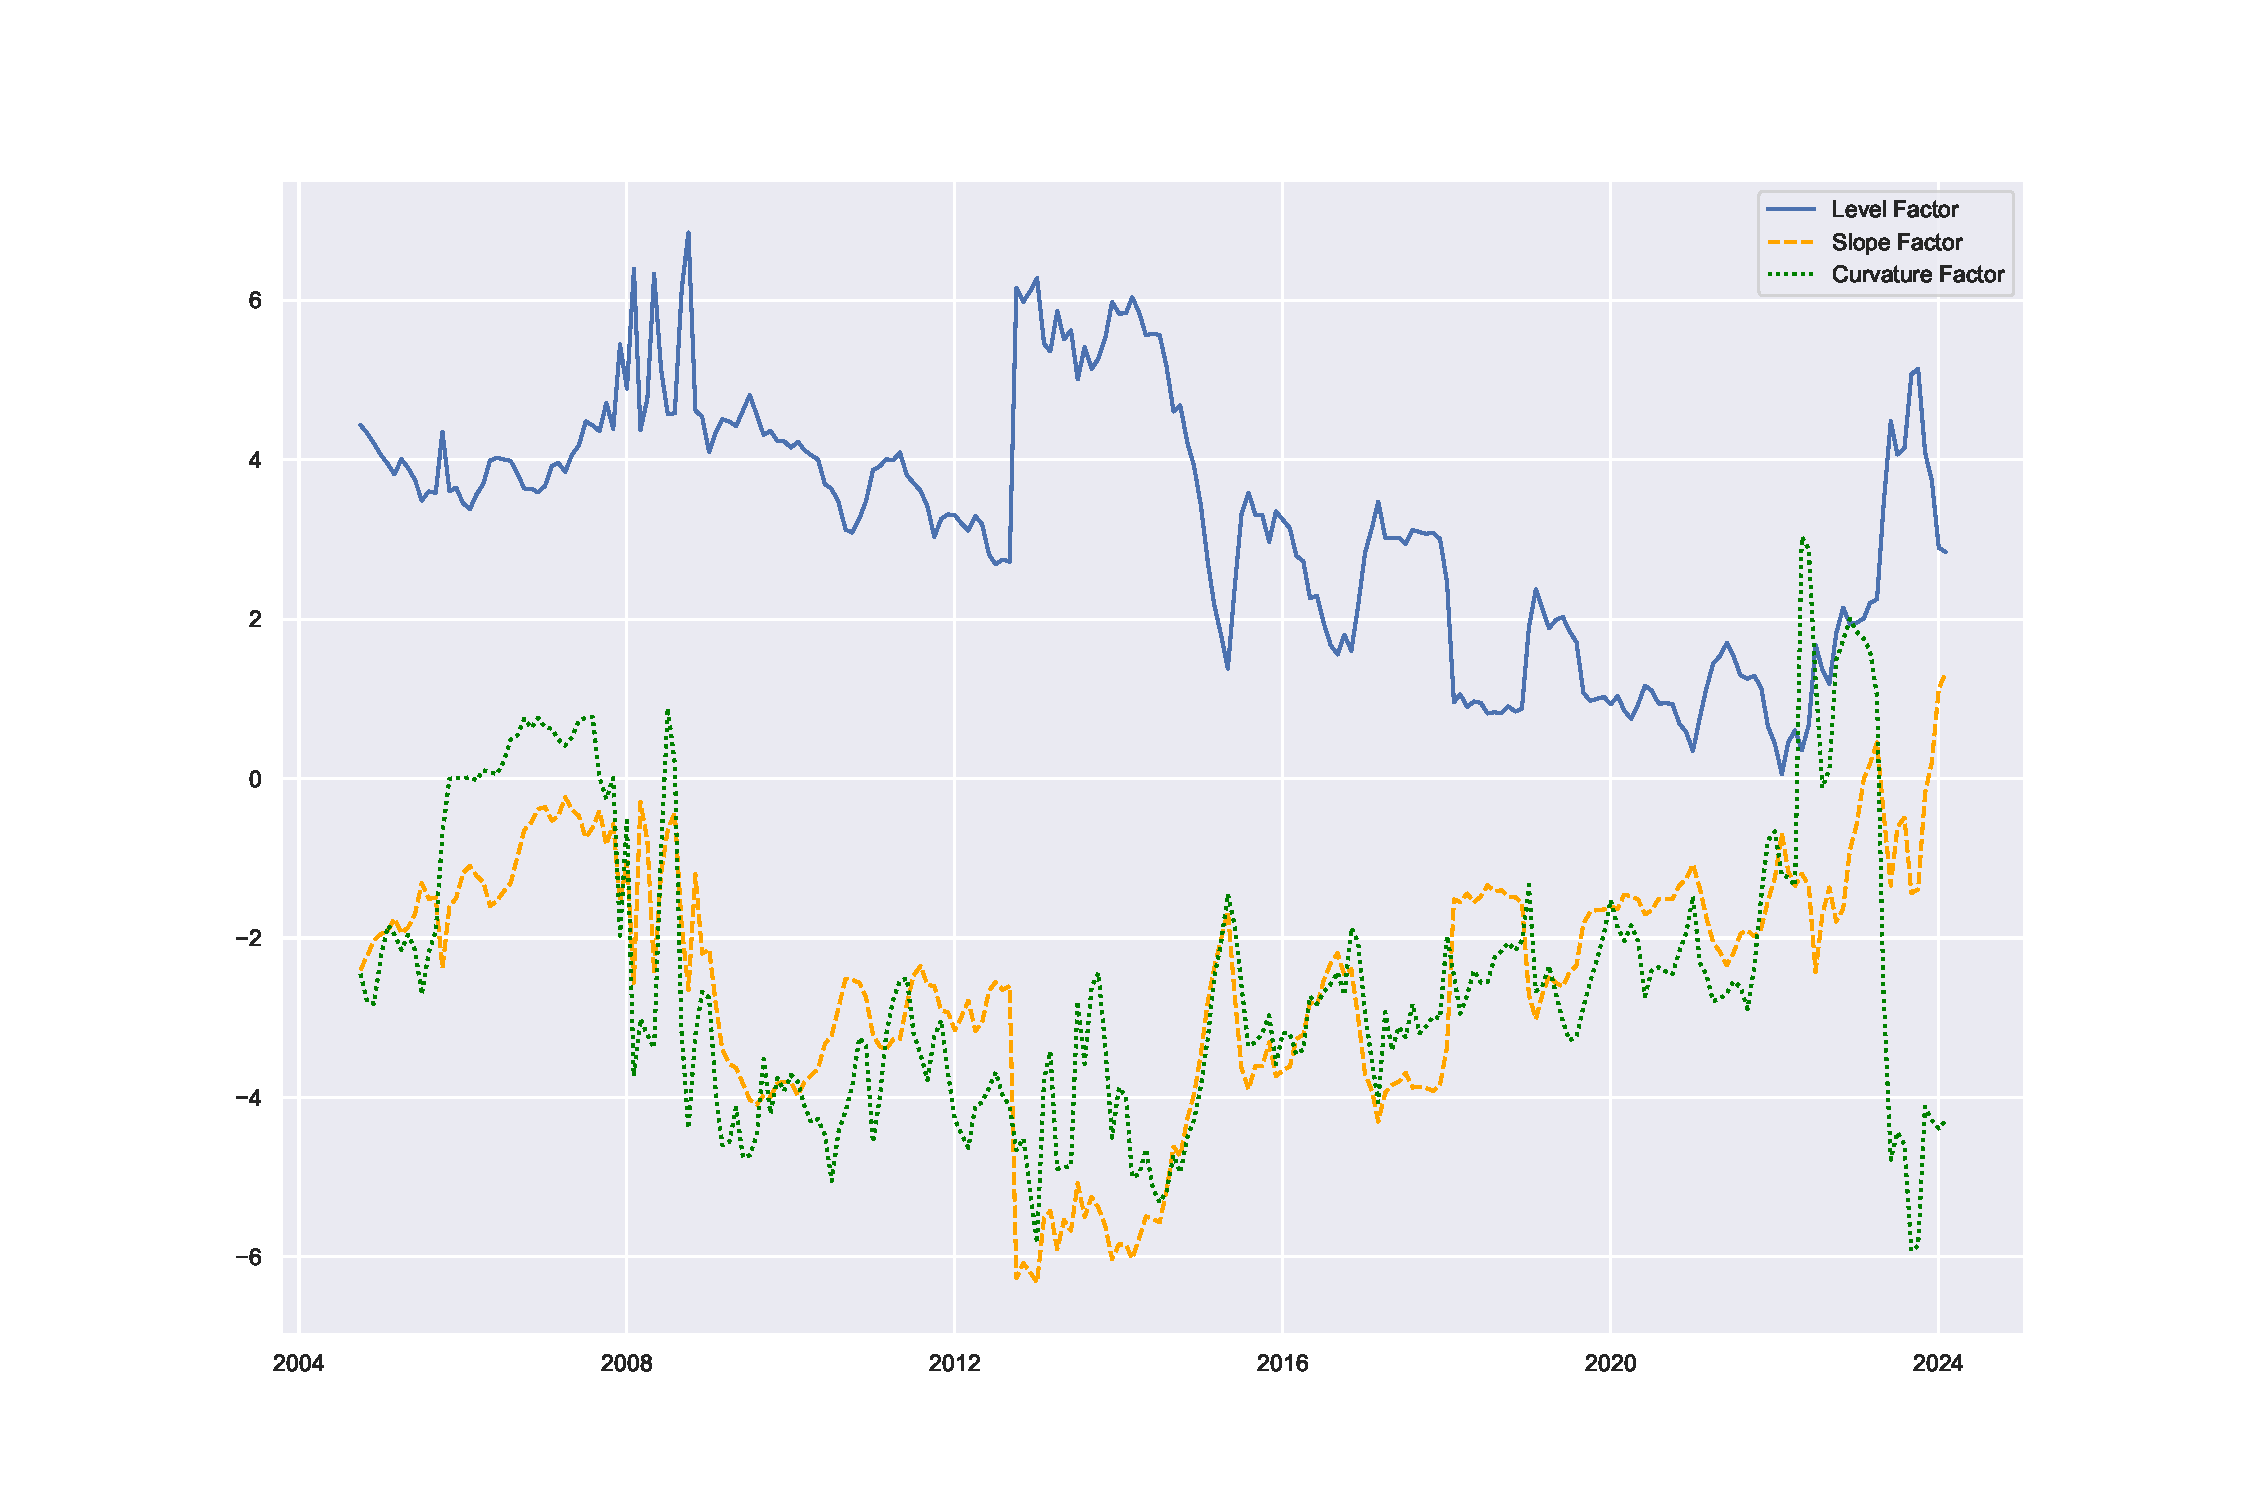
\includegraphics[width=15cm]{Figures/Factors_Figure_EA_1.pdf}
    \caption{Estimated level, slope and curvature factor, EA (in \%)}
    \label{fig:factors_ea}
\end{figure}

\begin{figure}[!t]
    \centering
    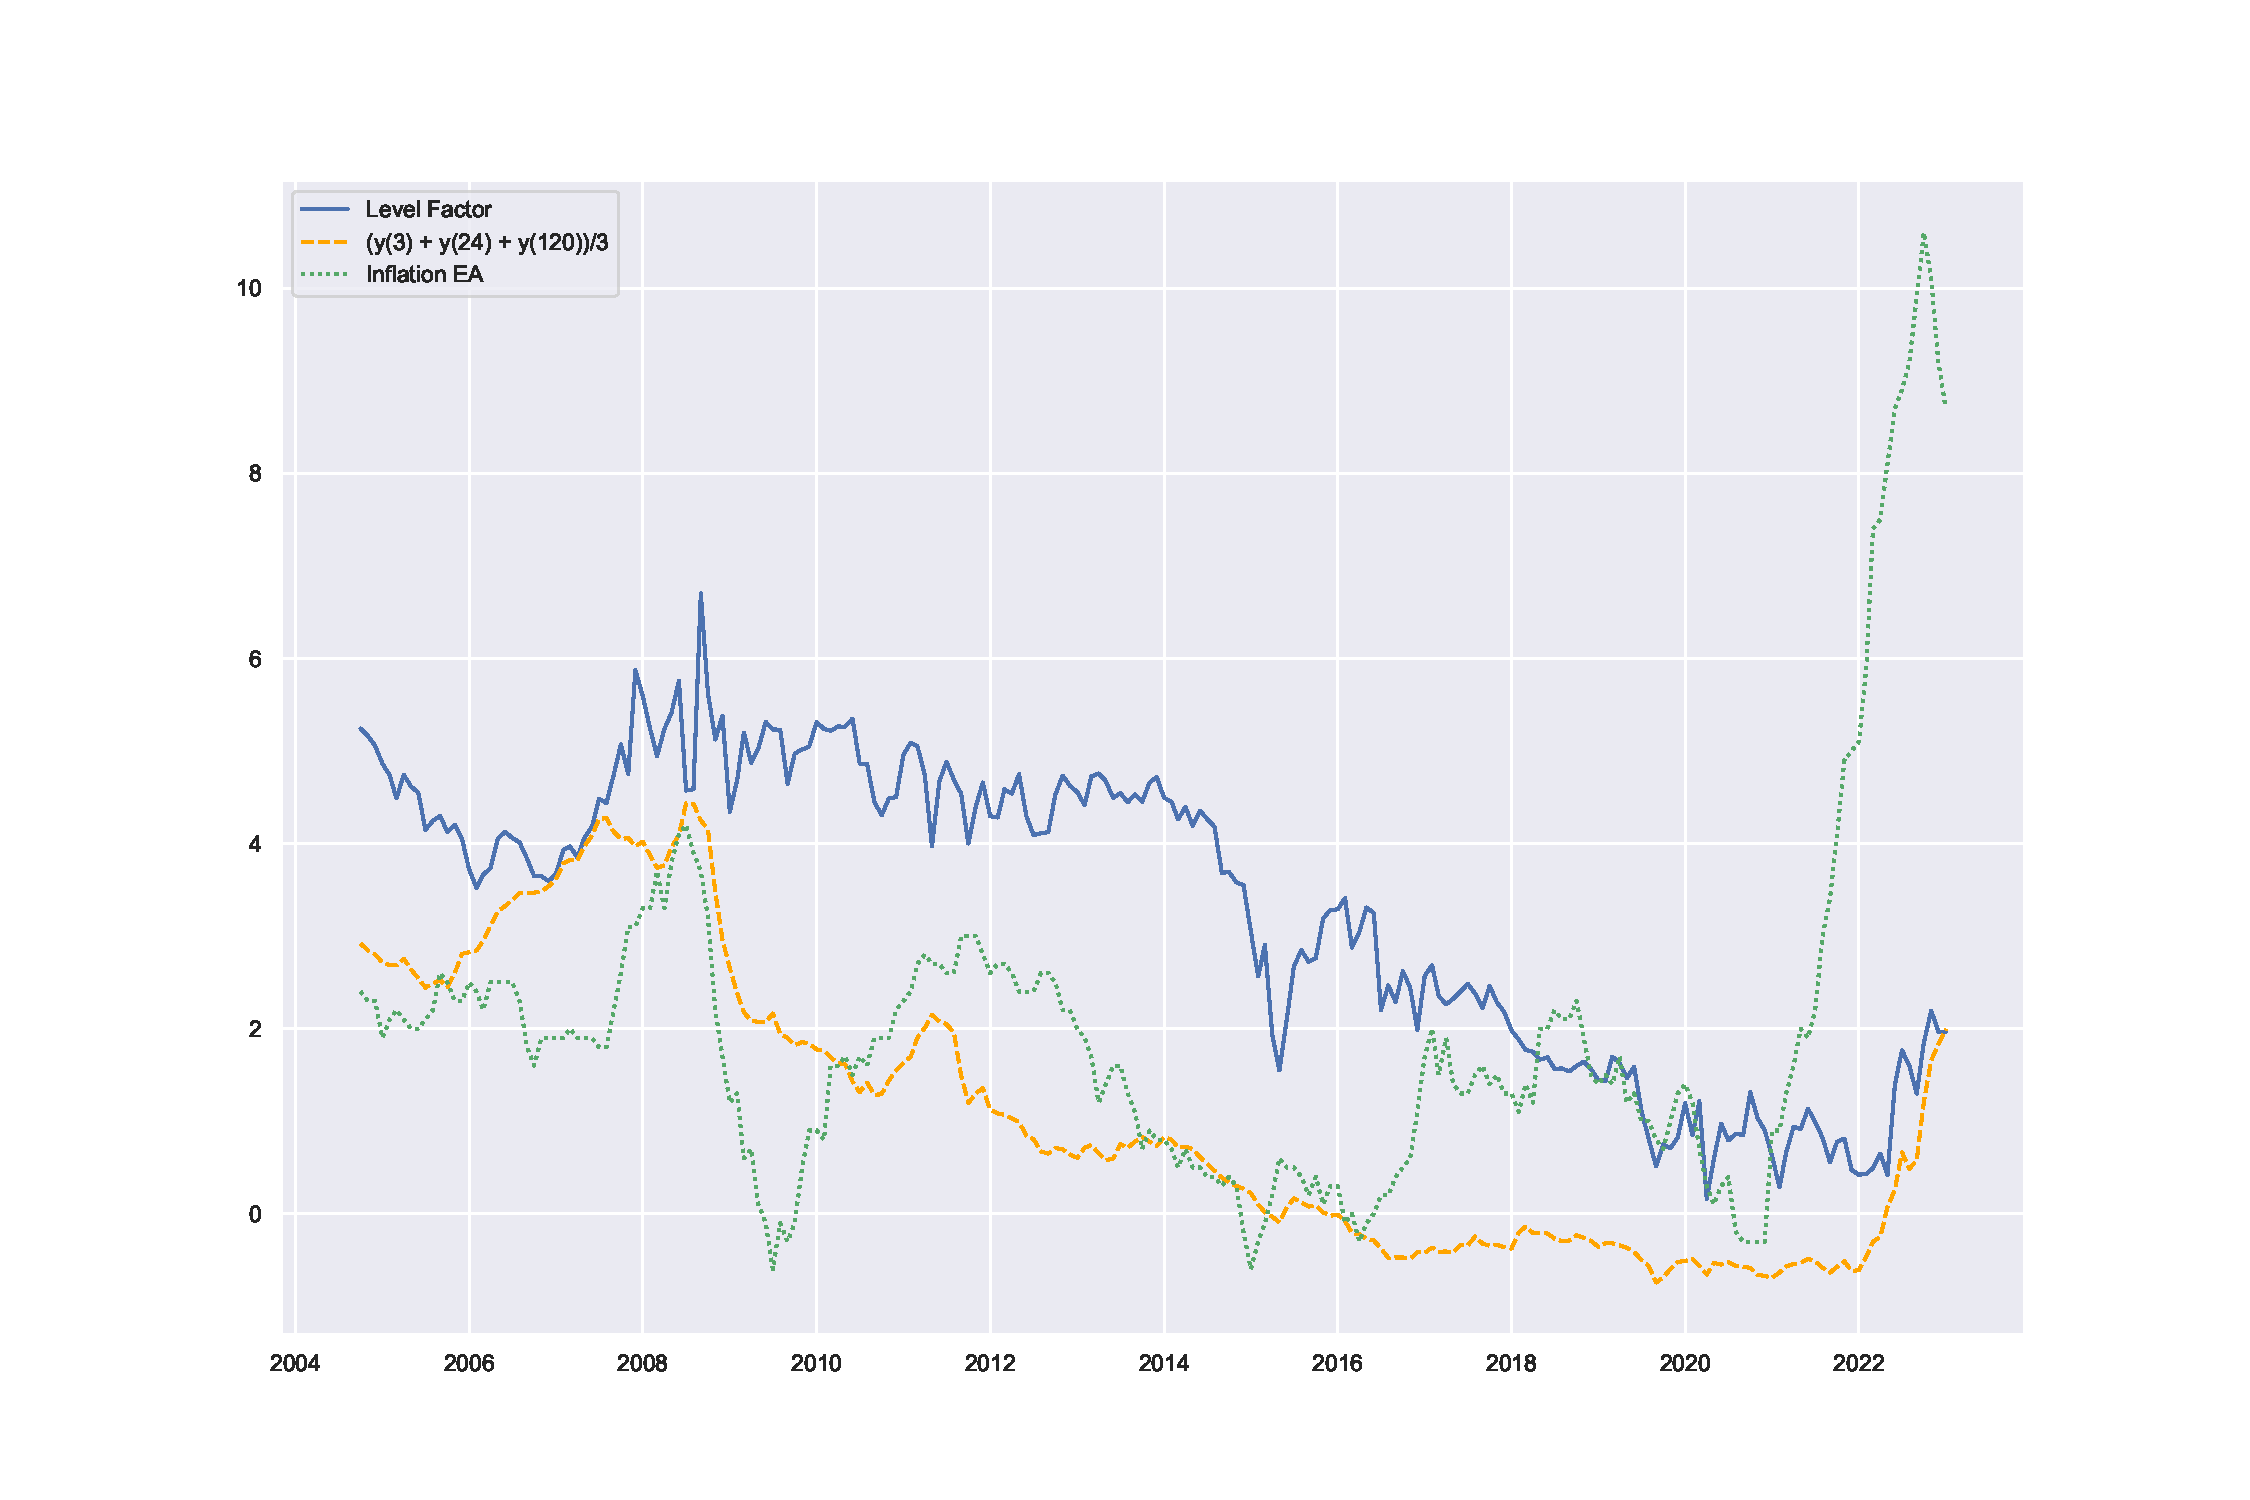
\includegraphics[width=15cm]{Figures/Beta_0_Figure_EA_1.pdf}
    \caption{Level factor, empirical proxy and inflation, EA (in \%)}
    \label{fig:level_factor_ea}
\end{figure}

\begin{figure}[!t]
    \centering
    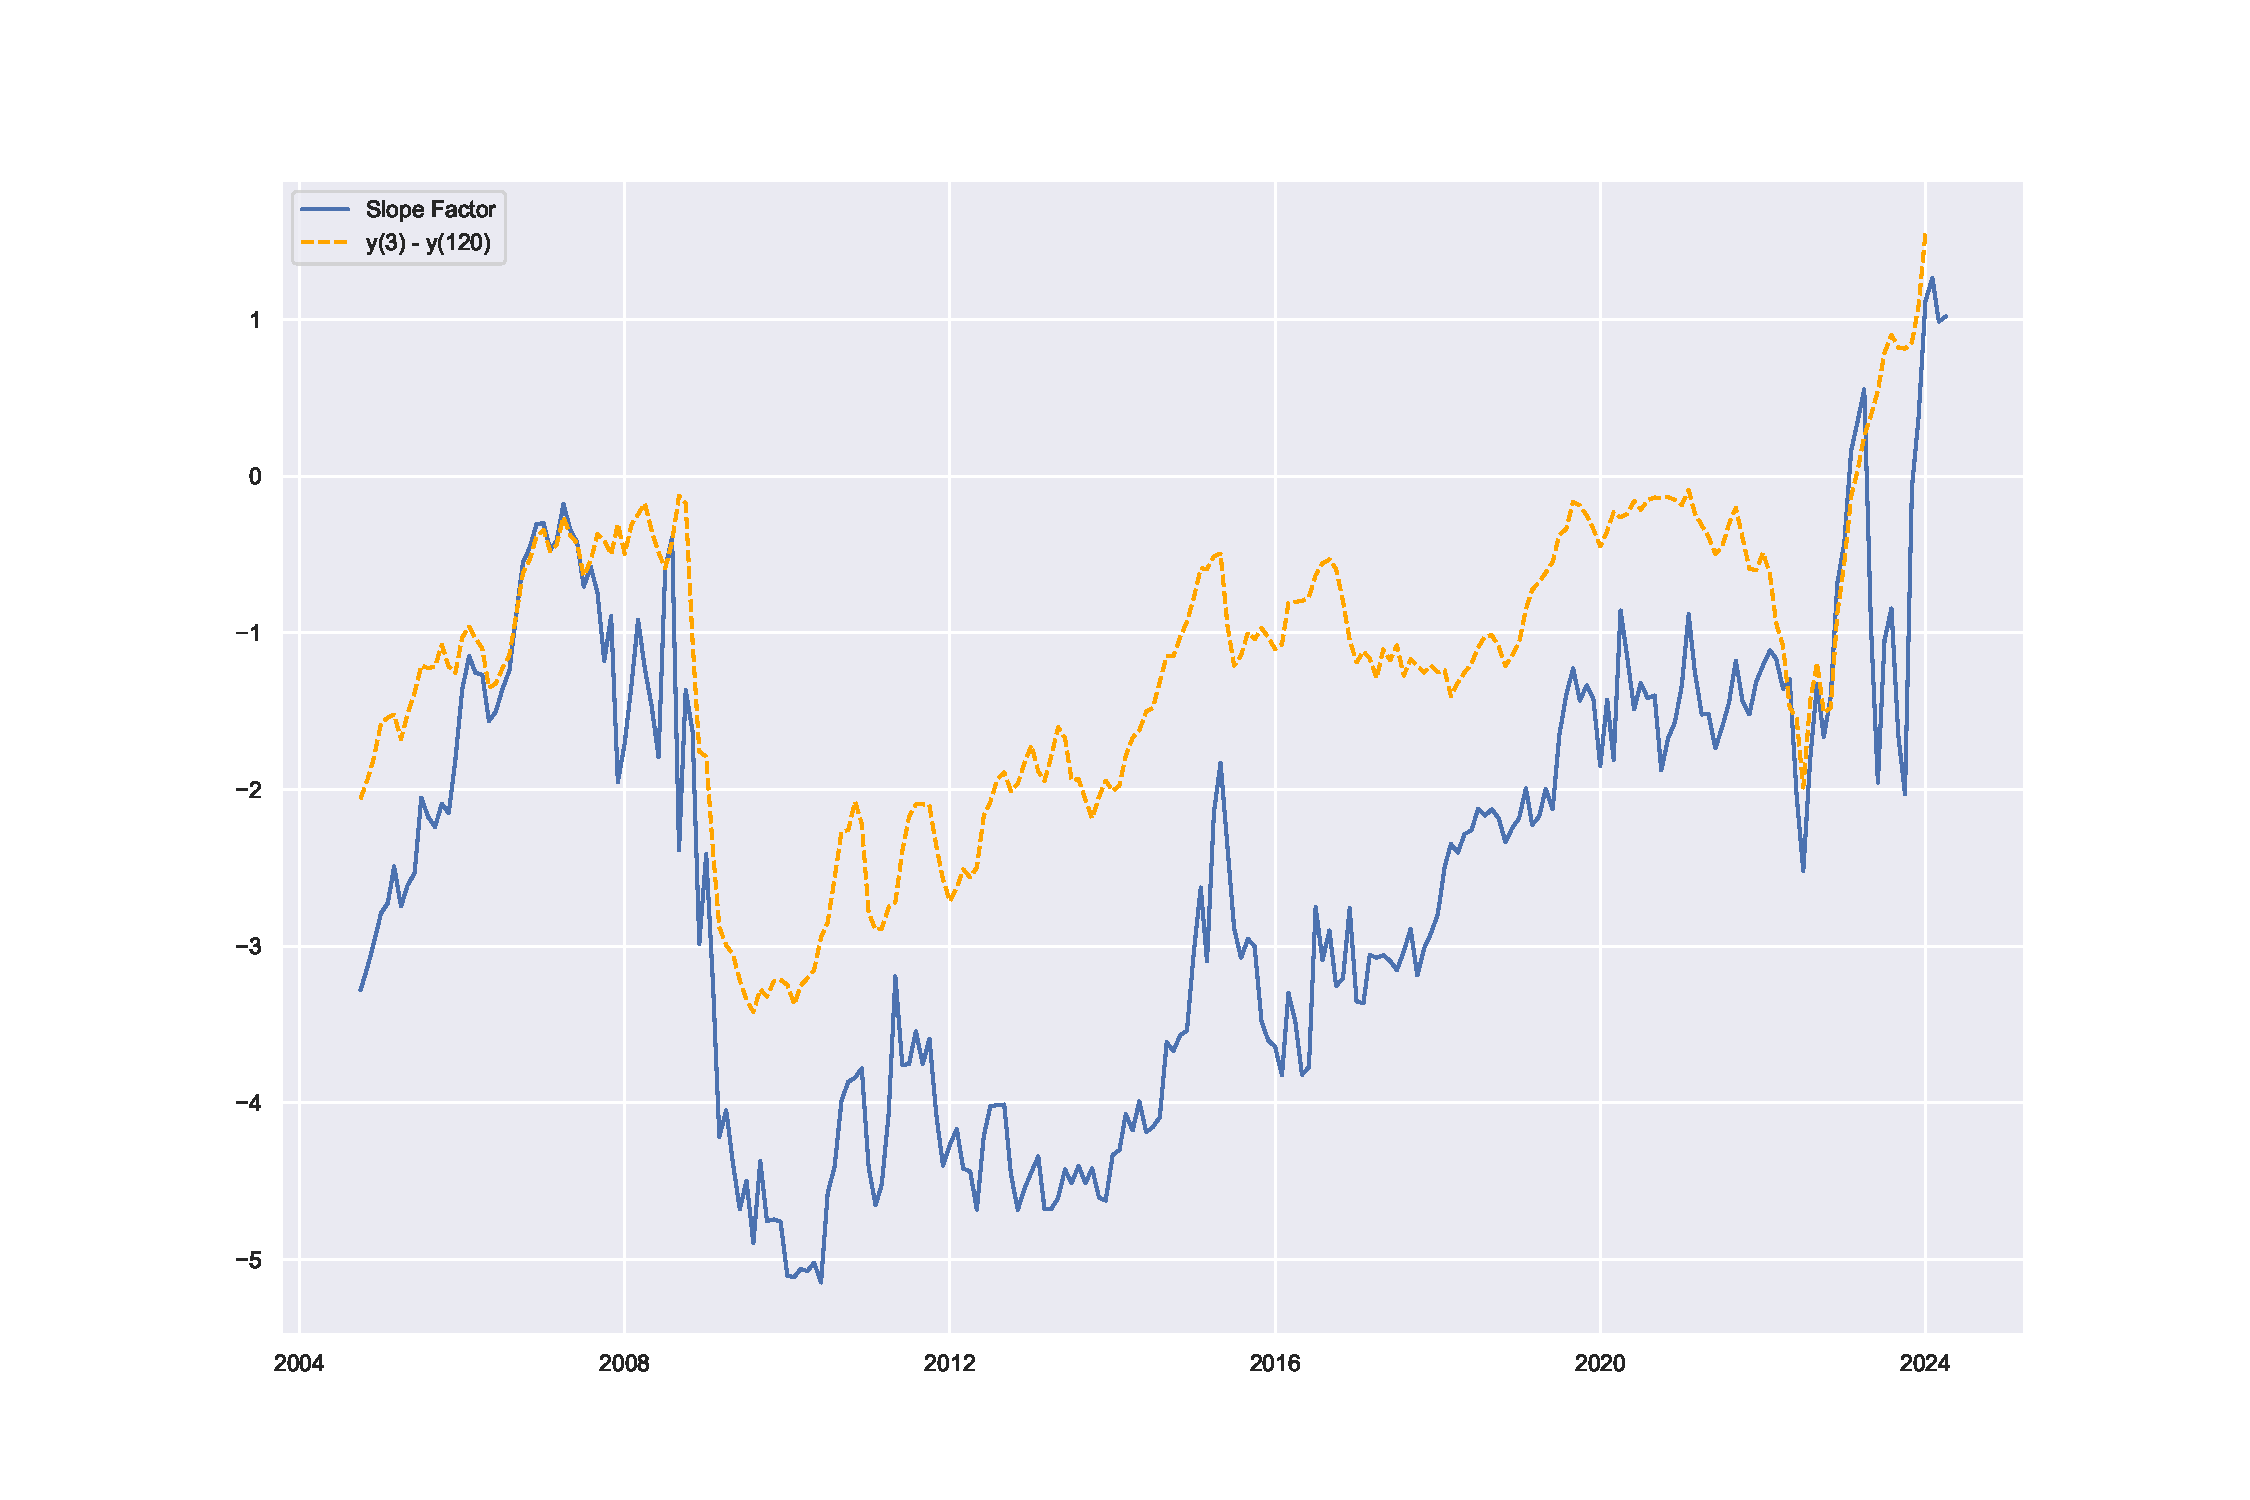
\includegraphics[width=15cm]{Figures/Beta_1_Figure_EA_1.pdf}
    \caption{Slope factor and empirical proxy, EA (in \%)}
    \label{fig:slope_factor_ea}
\end{figure}

\begin{figure}[!t]
    \centering
    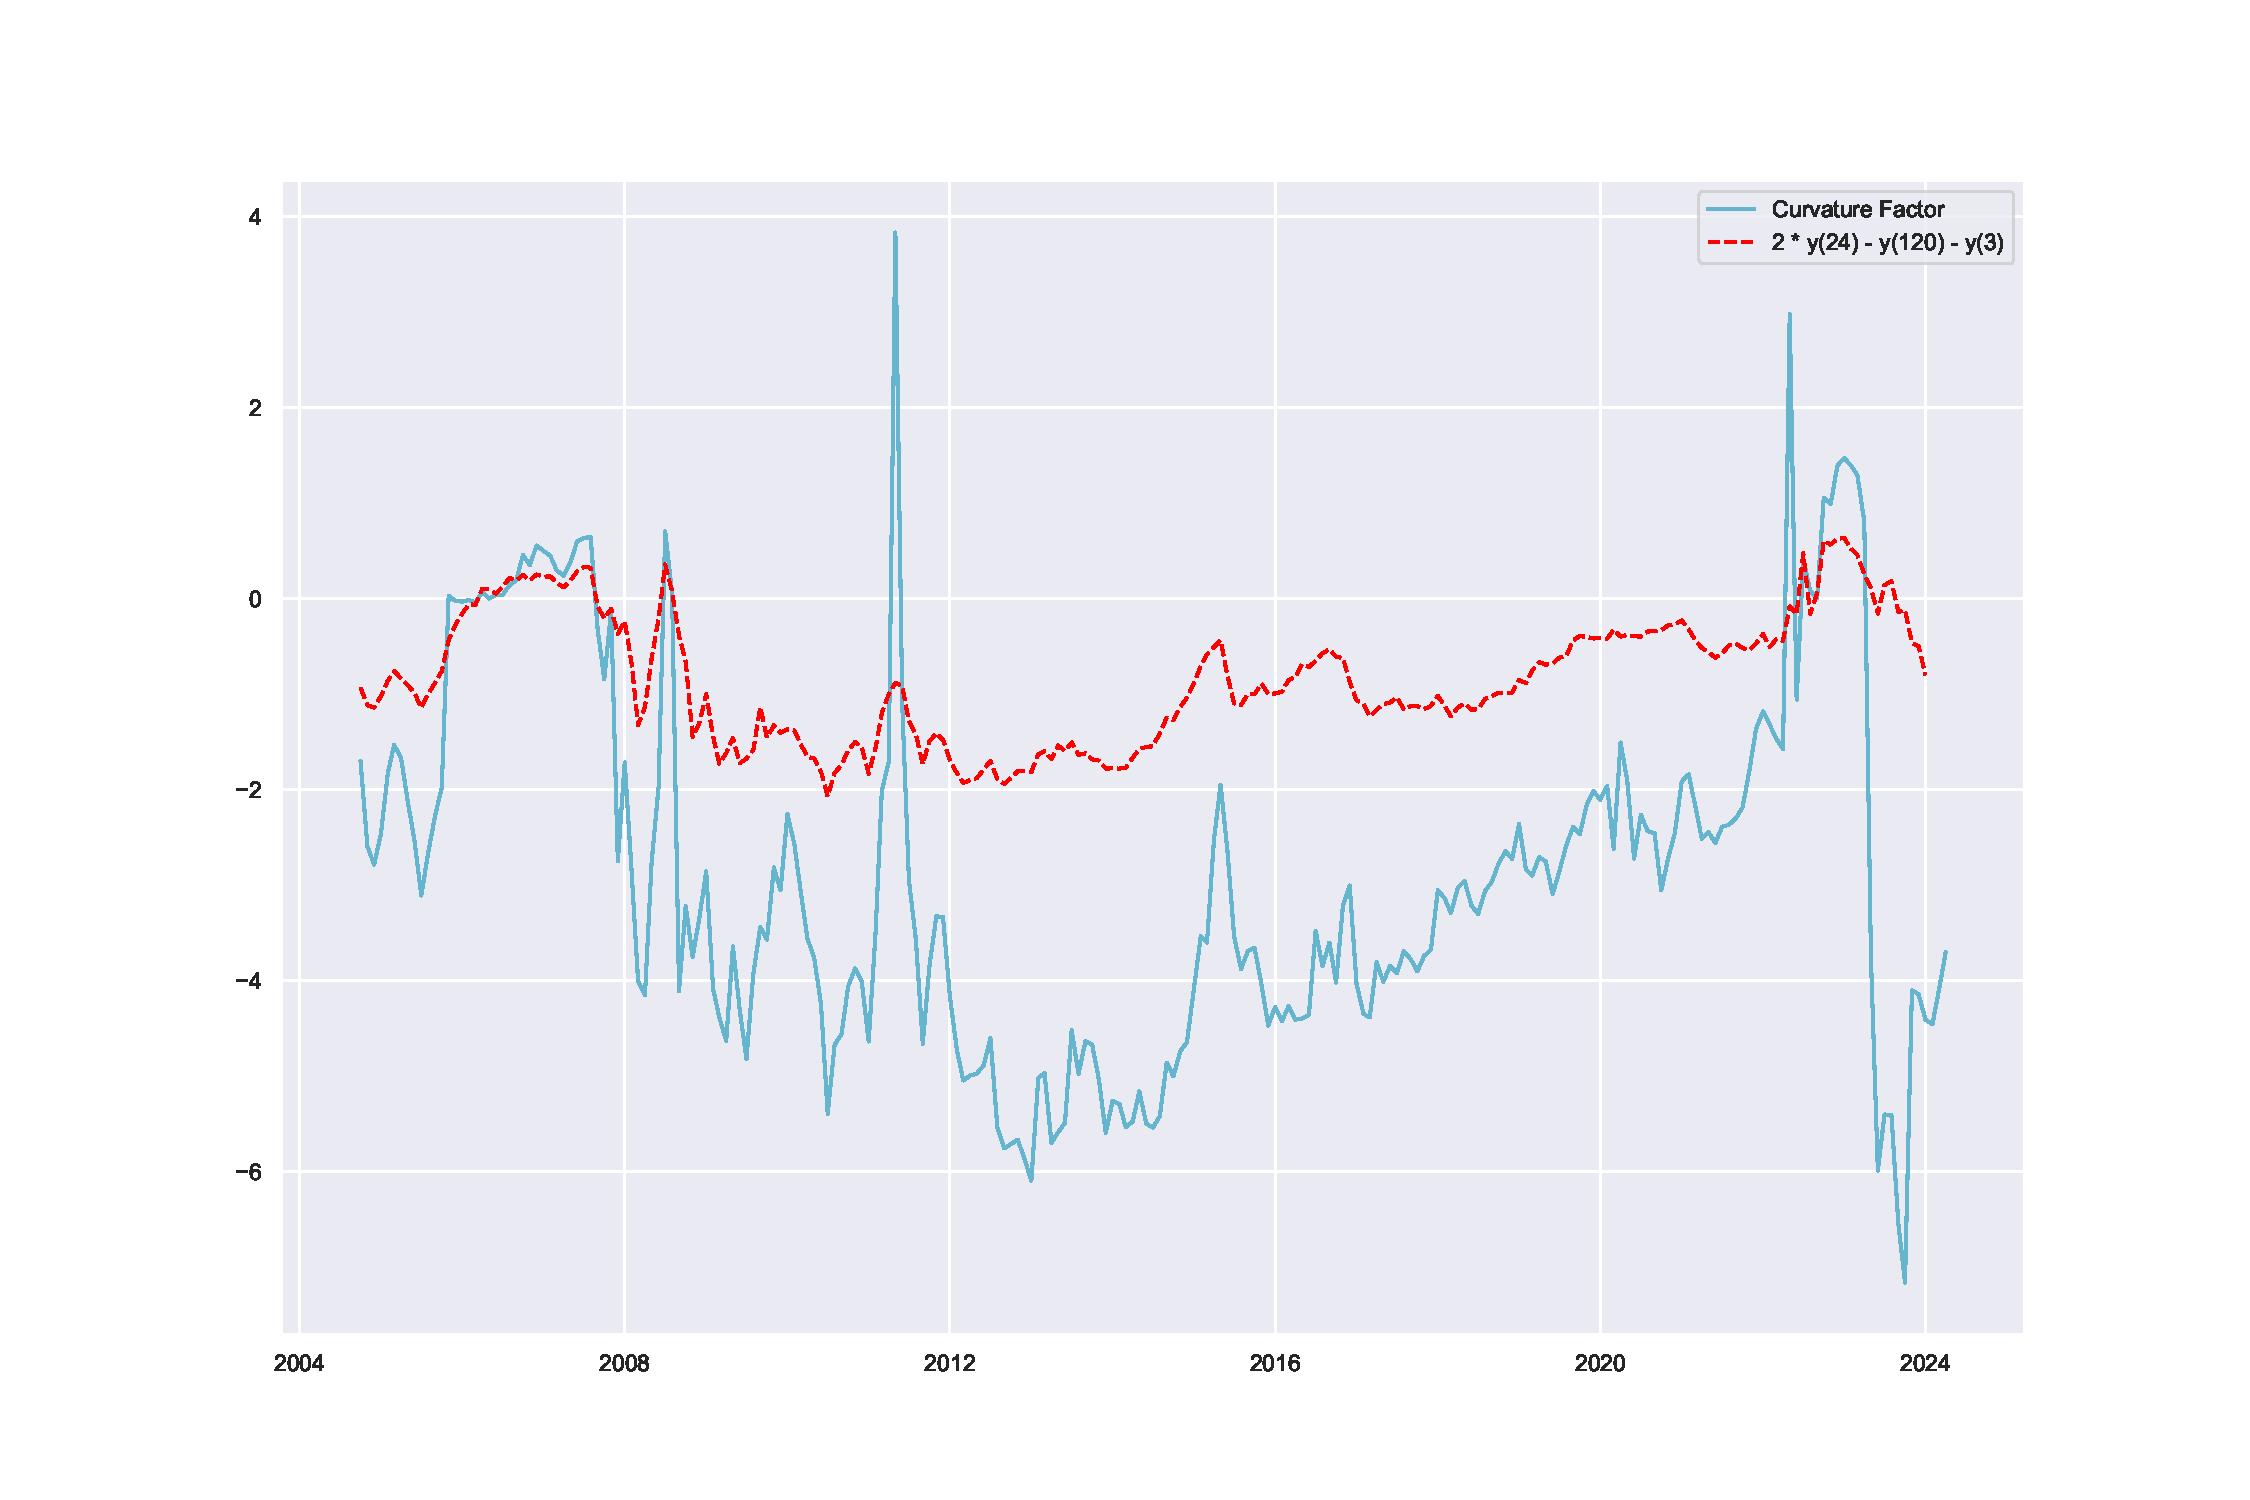
\includegraphics[width=15cm]{Figures/Beta_2_Figure_EA_1.pdf}
    \caption{Curvature factor and empirical proxy, EA (in \%)}
    \label{fig:curvature_factor_ea}
\end{figure}



Though, starting in January 2004, the sample period is markedly smaller compared to that of the United States, the analysis of the Euro Area nevertheless reveals some interesting insights into the relationship between the yield curve and the economy.
Again Figure \ref{fig:factors_ea} offers a comparison between all three estimated Nelson-Siegel factors over time.
Just like in the US, the level factor has been positive during the whole sample period, while also exhibiting a decreasing trend for most of the time, especially since the mid 2010s, a period, as mentioned before, marked by QE, negative interest rates, and in the case of the Euro Area, the European debt crisis. 
Since the start of 2022, where residual inflationary pressures due to the COVID-19 pandemic as well inflation induced by soaring energy prices due to the conflict in Ukraine also severely affected the European economy, the level factor has increased quite strongly, surpassing the 2\% mark - an interesting observation that is not only in line with the above mentioned Fisher effect regarding the relationship between the level effect and inflation, but this co-movement is also best seen in Figure \ref{fig:level_factor_ea}. 
With a correlation of 75\%, the slope factor displays a strong co-movement with the curvature factor. 
%Additionally, the slope factor approaches zero right at the onset of the financial crisis of 2007/08, an indication that it somewhat behaves in line with economic theory signaling a downturn when it inverts, though of course this is the only instance in the sample and by no means conclusive proof.
% Interestingly, $\hat{L}^{US}_{t}$, has been in positive territory since xx-2022, signalling an imminent recession, which was in this case a false positive. 
Evidently, the curvature factor has the highest volatility, especially due to the spike in  May 2011, which could again be due to an idiosyncratic shock in the form of the Euro crisis, but could also be attributed  to the fact that the Euro Area yields are based on a rather diverse pool of issuers with possible unobserved heterogeneity, which could potentially have confounding effects when using the Nelson-Siegel model.

Once more, in order to get an indication of how well the factor estimates represent the yield curve, Figures \ref{fig:level_factor_ea}-\ref{fig:curvature_factor_ea} display the estimated factors, $\hat{L}^{EA}_{t}$, $\hat{S}^{EA}_{t}$, $\hat{C}^{EA}_{t}$ with their respective empirical proxies. 
All three estimates exhibit a very strong and significant correlation with their proxies ranging from 74\% ($\hat{L}^{EA}_{t}$) to 86\% ($\hat{C}^{EA}_{t}$), which underlines the suitability of the estimates as accurately representing the level, slope and curvature of the Euro Area yield curve.
Most interestingly, the correlation between inflation and the level factor, though not being significant, is negative during the sample period, which of course contradicts the Fisher effect and the interpretation, that the level factor is an approximation for the expected inflation rate. Notably, not only is the sample period rather short, four highly idiosyncratic shocks have occurred during that short period of time, i.e. the financial crisis of 2007/08, the European debt crisis starting in 2010, the COVID-19 pandemic starting in 2020 and the ongoing war in Ukraine since February 2022, which likely stretches the rather simplistic approach used in this thesis to its limits. Adding to that the comparatively high heterogeneity of the Euro Area, it is by no means surprising to obtain counterintuitive results. 

Apart from the estimated slope factor and it's proxy variable, Figure \ref{fig:slope_factor_ea} also includes Euro Area industrial production representing economic activity. The first thing that stands out is the very high variability of industrial production, especially during the onset of the COVID-19 pandemic in early 2020, ranging from -19,91\% to 23,90\%. 
Though the recession following the financial crisis of 2007/08 was preceded by an upward trend of the estimated slope factor - being consistent with economic theory - the number of economic downturns simply is too small during the short sample to infer any substantial conclusions regarding the validity of the relationship between the term spread and economic activity in the Euro Area.

In short, Figures \ref{fig:factors_ea}-\ref{fig:curvature_factor_ea} show that the obtained estimates are very close to their respective proxy variables, and are thus well suited to represent the level, slope and curvature of the Euro Area yield curve. Nevertheless, they have also indicated that the limited sample period of 235 months marked by various distinct exogenous shocks impede to draw viable conclusions regarding the relationship between the yield curve and the macroeconomy in the Euro Area. 

% Again, the VAR model is estimated using OLS. 

% % \textbf{Correlation between factors, and approximations}

% \textbf{Granger Causality Tests?}

\begin{table}[t]
    \centering
    \begin{tabular}{lrrr}
        \toprule
        {} &  t-Statistic &  Critical value &  p-value \\
        \midrule
        $IP^{EA}_{t}$  &      -3.6453 &         -2.8757 &   0.0050 \\
        $\pi^{EA}_{t}$ &      -2.1955 &         -2.8757 &   0.2079 \\
        $i^{EA}_{t}$   &      -1.9314 &         -2.8756 &   0.3174 \\
        $FS^{EA}_{t}$  &      -5.0570 &         -2.8748 &   0.0000 \\
        $L^{EA}_{t}$   &      -1.0338 &         -2.8751 &   0.7407 \\
        $S^{EA}_{t}$   &      -1.3915 &         -2.8751 &   0.5863 \\
        $C^{EA}_{t}$   &      -1.5053 &         -2.8751 &   0.5309 \\
        $M^{EA}_{t}$   &      -3.5289 &         -2.8757 &   0.0073 \\
        \bottomrule
    \end{tabular}
    \caption{Augmented Dickey-Fuller (ADF) unit root test, EA}
    \label{tab:adf_ea}
\end{table}


\begin{sidewaystable}
    \centering
    \begin{tabular}{lrrrrrrrr}
        \toprule
        {} &        $IP^{EA}_{t}$ &   $\pi^{EA}_{t}$ &       $i^{EA}_{t}$ &       $FS^{EA}_{t}$ &         $\hat{L}^{EA}_{t}$ &         $\hat{S}^{EA}_{t}$ &         $\hat{C}^{EA}_{t}$ &   $M^{EA}_{t}$ \\
        \midrule
        const           &  1.2566 &   0.1349 &      0.1196 &  3.3488 &  0.0514 &  0.1131 & -0.3529 &    8.4328 \\
                &  (0.6388) &   (0.0985) &      (0.0355) &  (1.5143) &  (0.1072) &  (0.1115) &  (0.2697) &    (2.2158) \\
        $IP^{EA}_{t-1}$        &  0.8892 &   0.0156 &      0.0007 & -0.1784 & -0.0027 &  0.0017 & -0.0137 &    0.1437 \\
              &  (0.0422) &   (0.0065) &      (0.0023) &  (0.1001) &  (0.0071) &  (0.0074) &  (0.0178) &    (0.1465) \\
        $\pi^{EA}_{t-}$    & -0.0933 &   0.9983 &      0.0272 &  0.3455 & -0.0007 &  0.0135 &  0.1053 &   -0.7083 \\
            &  (0.0989) &   (0.0152) &      (0.0055) &  (0.2343) &  (0.0166) &  (0.0172) &  (0.0417) &    (0.3429) \\
        $i^{EA}_{t-1}$    & -0.5740 &  -0.0884 &      0.9627 &  1.5284 &  0.0275 &  0.0842 &  0.1549 &   -3.4139 \\
         &  (0.8192) &   (0.1263) &      (0.0455) &  (1.9419) &  (0.1375) &  (0.1429) &  (0.3458) &    (2.8416) \\
        $FS^{EA}_{t-1}$        & -0.0348 &   0.0030 &     -0.0056 &  0.7429 &  0.0042 & -0.0123 & -0.0093 &   -0.2087 \\
             &  (0.0230) &   (0.0036) &      (0.0013) &  (0.0546) &  (0.0039) &  (0.0040) &  (0.0097) &    (0.0799) \\
        $\hat{L}^{EA}_{t-1}$          &  0.4550 &   0.0404 &      0.0188 & -1.2571 &  0.9504 & -0.0918 & -0.1435 &    3.3983 \\
               &  (0.8775) &   (0.1353) &      (0.0488) &  (2.0801) &  (0.1473) &  (0.1531) &  (0.3704) &    (3.0438) \\
        $\hat{S}^{EA}_{t-1}$          &  0.0760 &   0.0605 &     -0.0022 & -1.0454 & -0.0330 &  0.8605 &  0.0540 &    2.0348 \\
               &  (0.8234) &   (0.1269) &      (0.0457) &  (1.9517) &  (0.1382) &  (0.1436) &  (0.3476) &    (2.8559) \\
        $\hat{C}^{EA}_{t-1}$          &  0.3245 &   0.0258 &      0.0317 & -0.5248 &  0.0417 &  0.0015 &  0.7142 &    1.1557 \\
               &  (0.1359) &   (0.0210) &      (0.0076) &  (0.3222) &  (0.0228) &  (0.0237) &  (0.0574) &    (0.4715) \\
        $M^{EA}_{t-1}$      & -0.0024 &   0.0002 &      0.0013 &  0.0383 &  0.0011 & -0.0002 &  0.0051 &    0.8038 \\
           &  (0.0126) &   (0.0019) &      (0.0007) &  (0.0299) &  (0.0021) &  (0.0022) &  (0.0053) &    (0.0437) \\
    \midrule
    Log-Likelihood & -1759.3817 \\
    AIC            &    -5.9781 \\
    BIC            &    -4.8639 \\
    HQIC           &    -5.5281 \\
    \bottomrule
    \end{tabular}
    \caption{Vector Autoregression estimation results, EA}
    \label{tab:VAR_output_EA}
\end{sidewaystable}


\begin{sidewaysfigure}
    \centering
    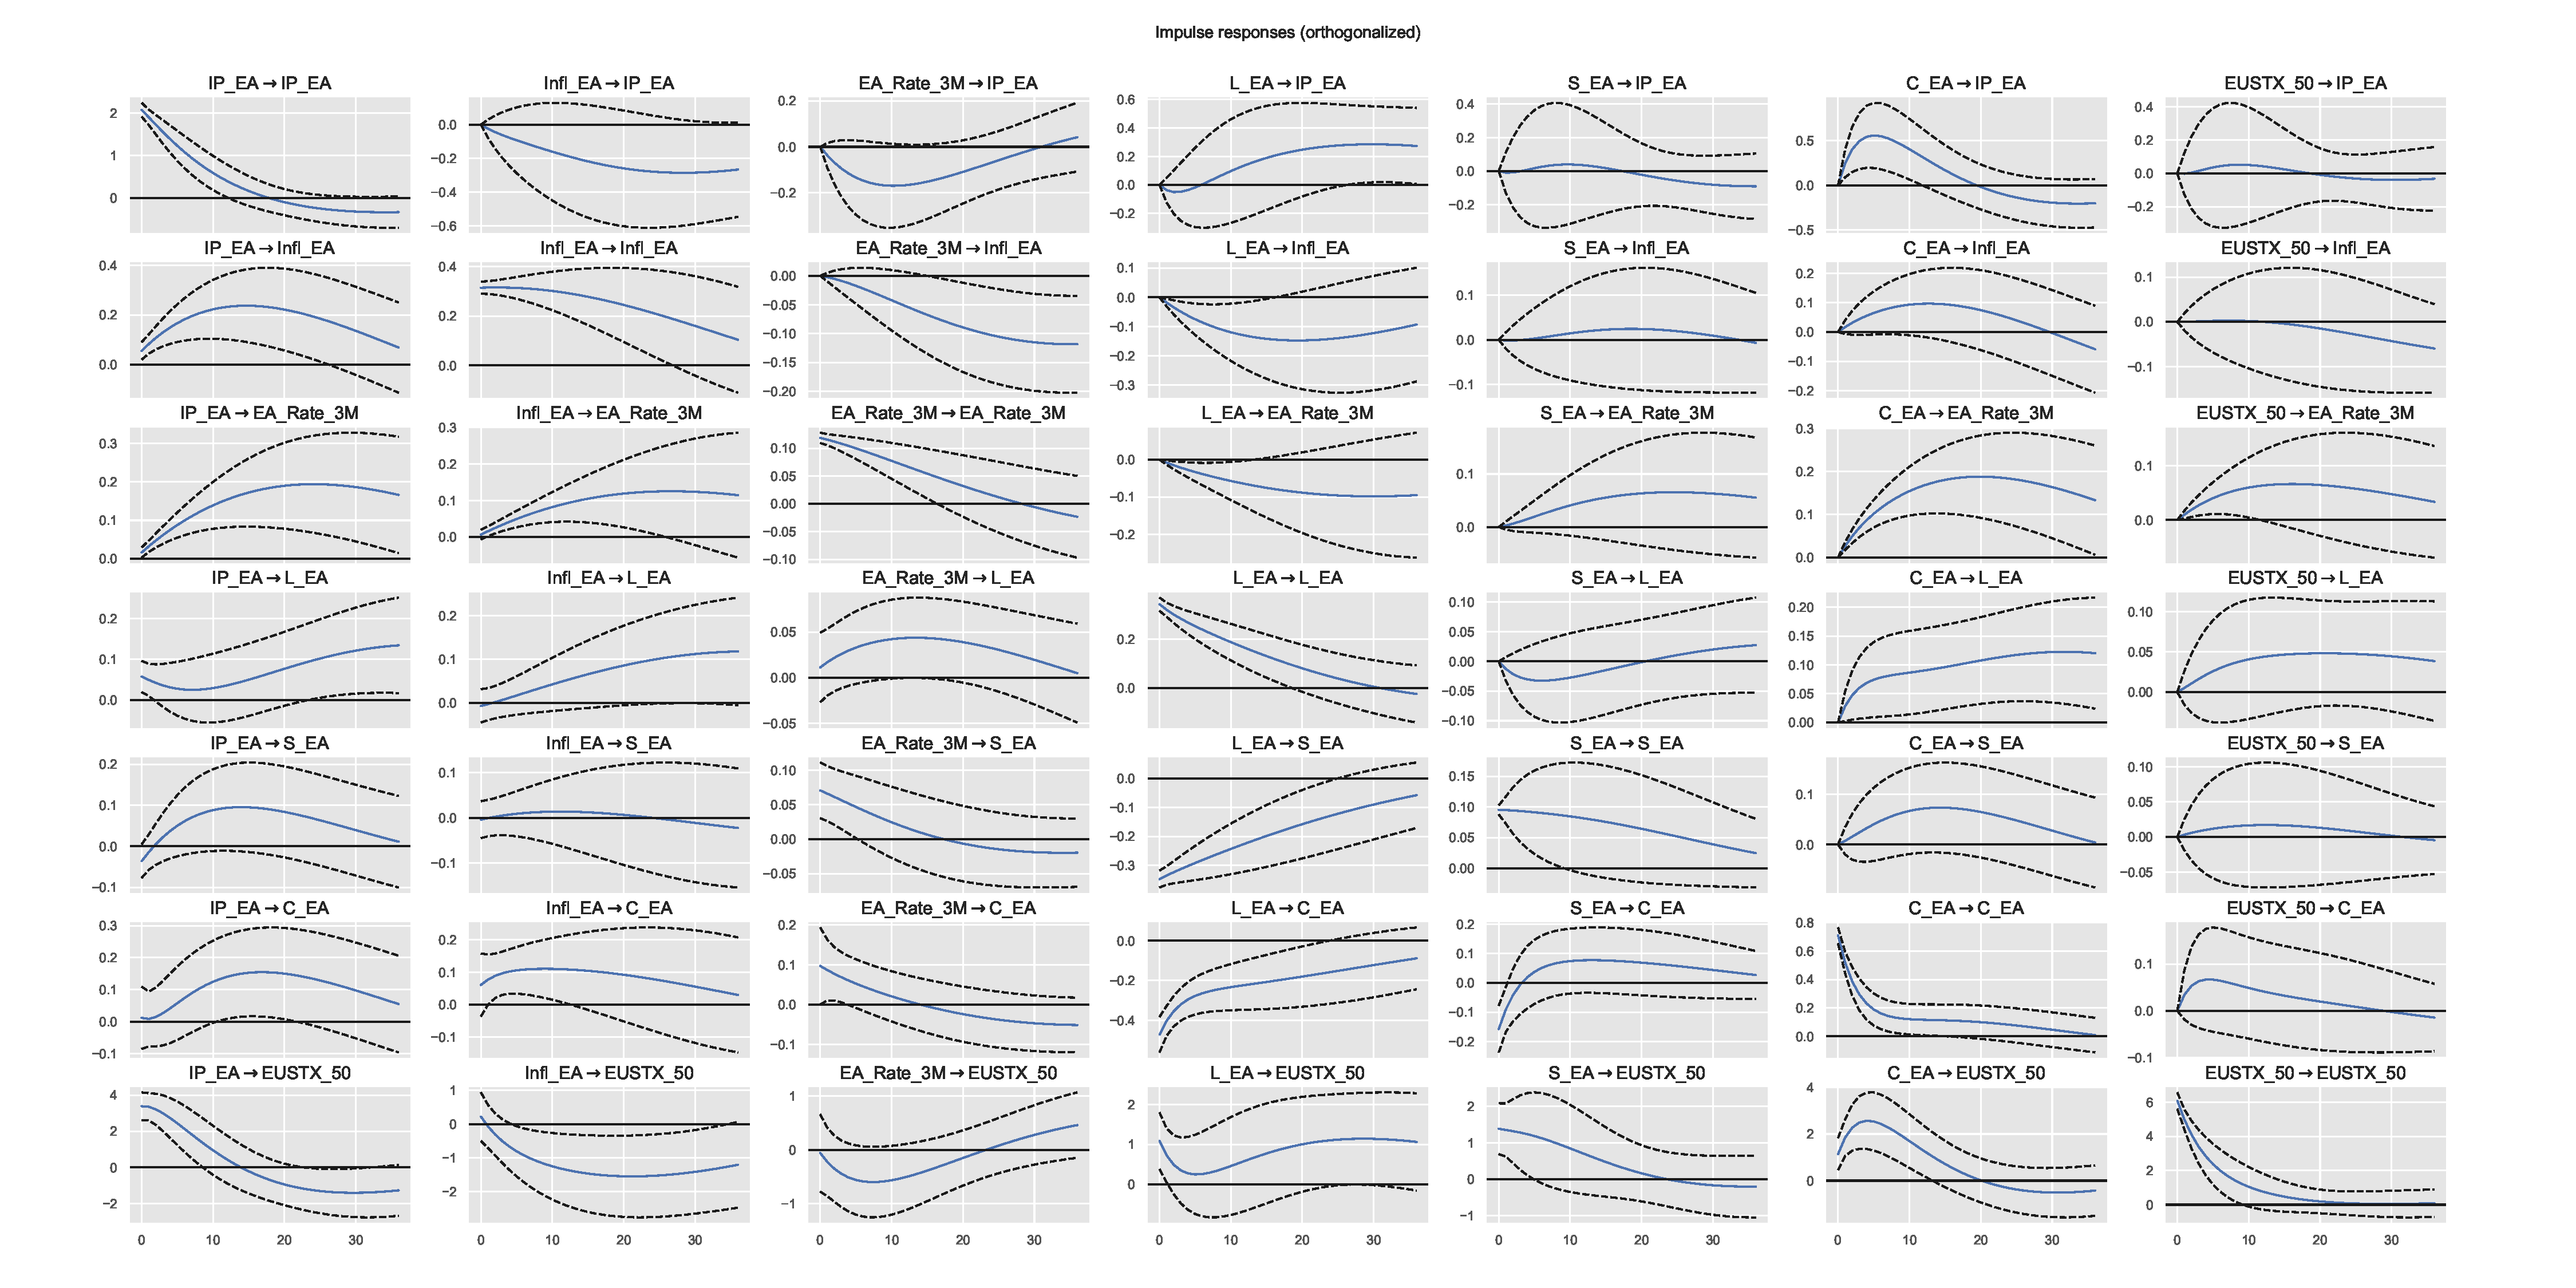
\includegraphics[scale=0.29]{Figures/IRF_EA_30_15_v2.pdf}
    \caption{Impulse Responses, EA}
    \label{fig:IRF_EA}
\end{sidewaysfigure}

\begin{table}[!t]
    \centering
    \begin{tabular}{lllll}
    \toprule
    {} &     t-statistic &      Critical value &                 p-value 
    \\
    \midrule
    Macro-to-Yields &  3.5250 &  1.8854 &  0.0002 &  \\
    % \midrule
    Yields-to-Macro &   3.3156 &  1.8854 &  0.0005  \\
\bottomrule
    \end{tabular}
    \caption{Block Granger causality tests, EA}
    \label{tab:granger_ea}
\end{table}









